% This LaTeX was auto-generated from MATLAB code.
% To make changes, update the MATLAB code and export to LaTeX again.

\documentclass{article}

\usepackage[utf8]{inputenc}
\usepackage[T1]{fontenc}
\usepackage{lmodern}
\usepackage{graphicx}
\usepackage{color}
\usepackage{listings}
\usepackage{hyperref}
\usepackage{amsmath}
\usepackage{amsfonts}
\usepackage{epstopdf}
\usepackage{matlab}

\sloppy
\epstopdfsetup{outdir=./}
\graphicspath{ {./transferring_a_robot_sol_images/} }

\begin{document}

\matlabtitle{1. Transferring a robot}


\matlabheading{1.0 Initialization}

\begin{matlabcode}
clear;
\end{matlabcode}


\matlabheading{1.1 The setup}

\begin{matlabcode}
% Given dynamics matrices 
A = [1  0   0.1   0;...
     0  1   0     0.1;...
     0  0   0.9   0;...
     0  0   0     0.9];
B = [0   0;...
     0   0;...
     0.1 0;...
     0   0.1];
n = 4;
m = 2; 

% Given parameters
T = 80;
p_initial = [0;5];
p_final = [15;-15];
w = [10 10; 20 10; 30 10; 30 0; 20 0; 10 -10]';
tau = [10 25 30 40 50 60];
U_max = 100;
E = [eye(2) zeros(2)];
\end{matlabcode}


\matlabheading{1.2 The $l_2^2$ regularizer}

\begin{matlabcode}
controlSignalChanges = [];
meanDeviation = [];

for lambda_log = -3:3
    % ---------- Setup optimization problem ----------
    cvx_begin quiet
        % optimization variables
        variables x(n,T+1) u(m,T)
        % cost function
        minimize(sum(sum_square(E*x(:,tau+1)-w))+...
            (10^lambda_log)*sum(sum_square(u*(diag(-[ones(T-1,1);0])+diag(ones(T-1,1),-1)))));
        % subject to
        x(:,1) == [p_initial;zeros(2,1)];
        x(:,end) == [p_final;zeros(2,1)];
        for t = 1:T
            x(:,t+1) == A*x(:,t)+B*u(:,t);
            norm(u(:,t)) <= U_max;
        end
    cvx_end
    
    % ---------- Plot result ----------
    % trajectory
    figure('units','normalized','outerposition',[0 0 1 1]);
    hold on;
    set(gca,'FontSize',35);
    ax = gca;
    ax.XGrid = 'on';
    ax.YGrid = 'on';
    axis equal;
    title(strcat('$1.2\;a)\; \mathrm{Trajectory}\;\lambda =',sprintf('10^{%d}$',lambda_log)),'Interpreter','latex');
    scatter(x(1,:),x(2,:),70,'o','blue','LineWidth',3);
    scatter(x(1,tau+1),x(2,tau+1),300,'o','magenta','LineWidth',4);
    scatter(w(1,:),w(2,:),300,'s','red','LineWidth',4);
    legend('Trajectory','Waypoints (followed)', 'Waypoints (desired)','Location','best');
    ylabel('$p_y$','Interpreter','latex');
    xlabel('$p_x$','Interpreter','latex');
    saveas(gcf,sprintf('./transferring_a_robot_data/1_2_trajectory_1e%d.fig',lambda_log));
    saveas(gcf,sprintf('./transferring_a_robot_data/1_2_trajectory_1e%d.png',lambda_log));
    hold off; 
    
    % control signal
    figure('units','normalized','outerposition',[0 0 1 1]);
    hold on;
    set(gca,'FontSize',35);
    ax = gca;
    ax.XGrid = 'on';
    ax.YGrid = 'on';
    axis equal;
    title(strcat('$1.2\;b)\; \mathrm{Control}\;\mathrm{signal}\;\lambda =',sprintf('10^{%d}$',lambda_log)),'Interpreter','latex');
    scatter(0:T-1,u(1,:),70,'o','LineWidth',3);
    scatter(0:T-1,u(2,:),70,'o','LineWidth',3);
    legend({'$\mathbf{u}_1(t)$','$\mathbf{u}_2(t)$'},'Location','best','interpreter','latex');
    ylabel('$ $','Interpreter','latex');
    xlabel('$t$','Interpreter','latex');
    saveas(gcf,sprintf('./transferring_a_robot_data/1_2_controlSignal_1e%d.fig',lambda_log));
    saveas(gcf,sprintf('./transferring_a_robot_data/1_2_controlSignal_1e%d.png',lambda_log));
    hold off;
    
    controlSignalChangesCur = 0;
    for t = 1:T-1
        if norm(u(:,t+1)-u(:,t))>1e-4
            controlSignalChangesCur = controlSignalChangesCur+1;
        end
    end
    controlSignalChanges = [controlSignalChanges [10^lambda_log;controlSignalChangesCur]]; 
    fprintf("1.2 c) For lambda = 1e%d there were %d optimal control signal changes.\n",lambda_log,controlSignalChangesCur);
    
    meanDeviationCur = (1/length(w))*sum(sqrt(sum_square(E*x(:,tau+1)-w)));
    meanDeviation = [meanDeviation [10^lambda_log; meanDeviationCur]];
    fprintf("1.2 d) For lambda = 1e%d the mean deviation from the waypoints is %f.\n",lambda_log,meanDeviationCur);
end
\end{matlabcode}
\begin{center}
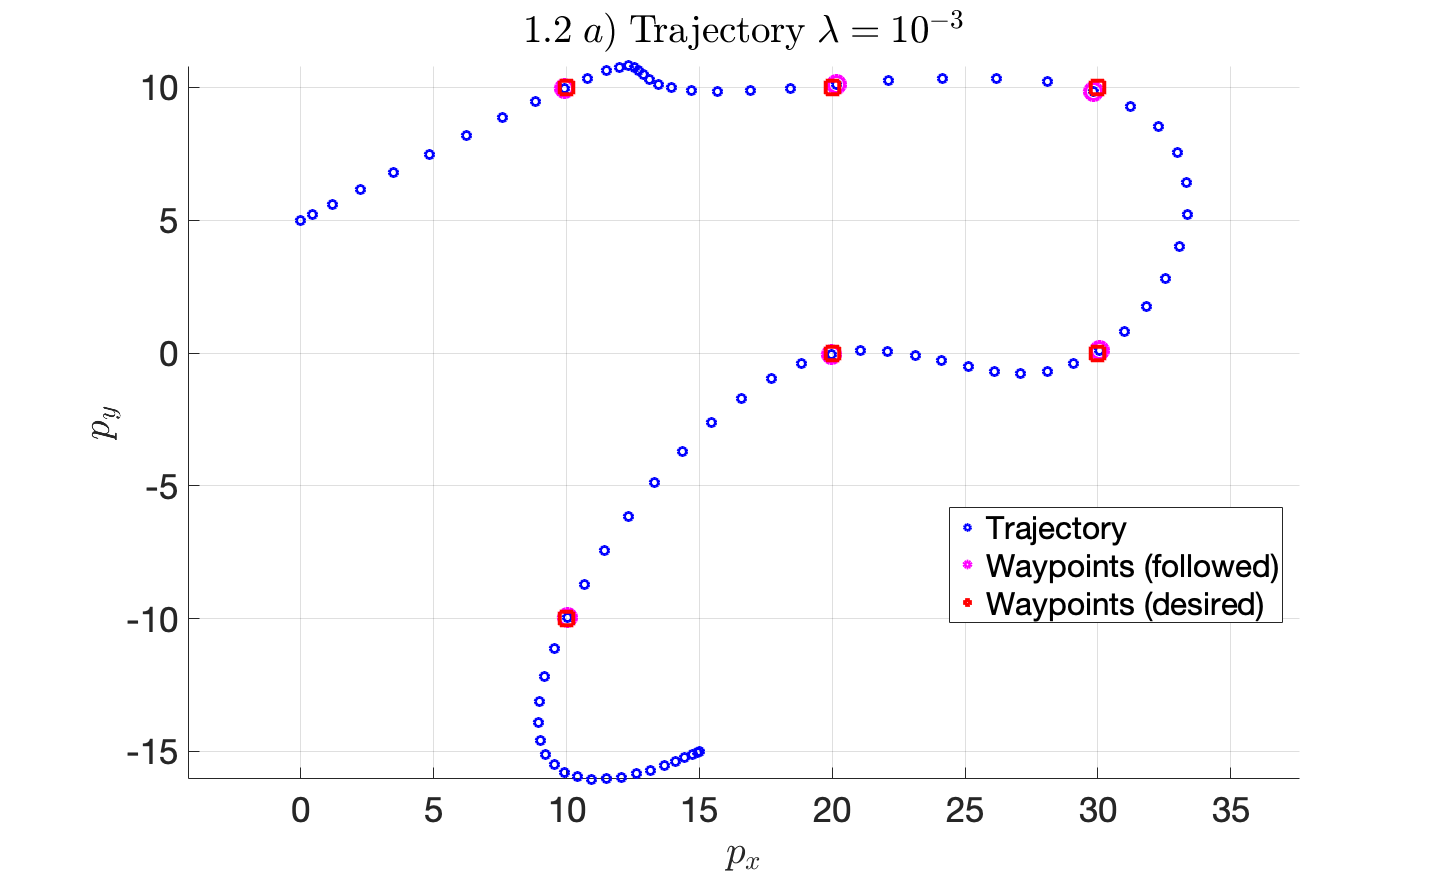
\includegraphics[width=\maxwidth{144.5057701956849em}]{figure_0}
\end{center}

\begin{center}
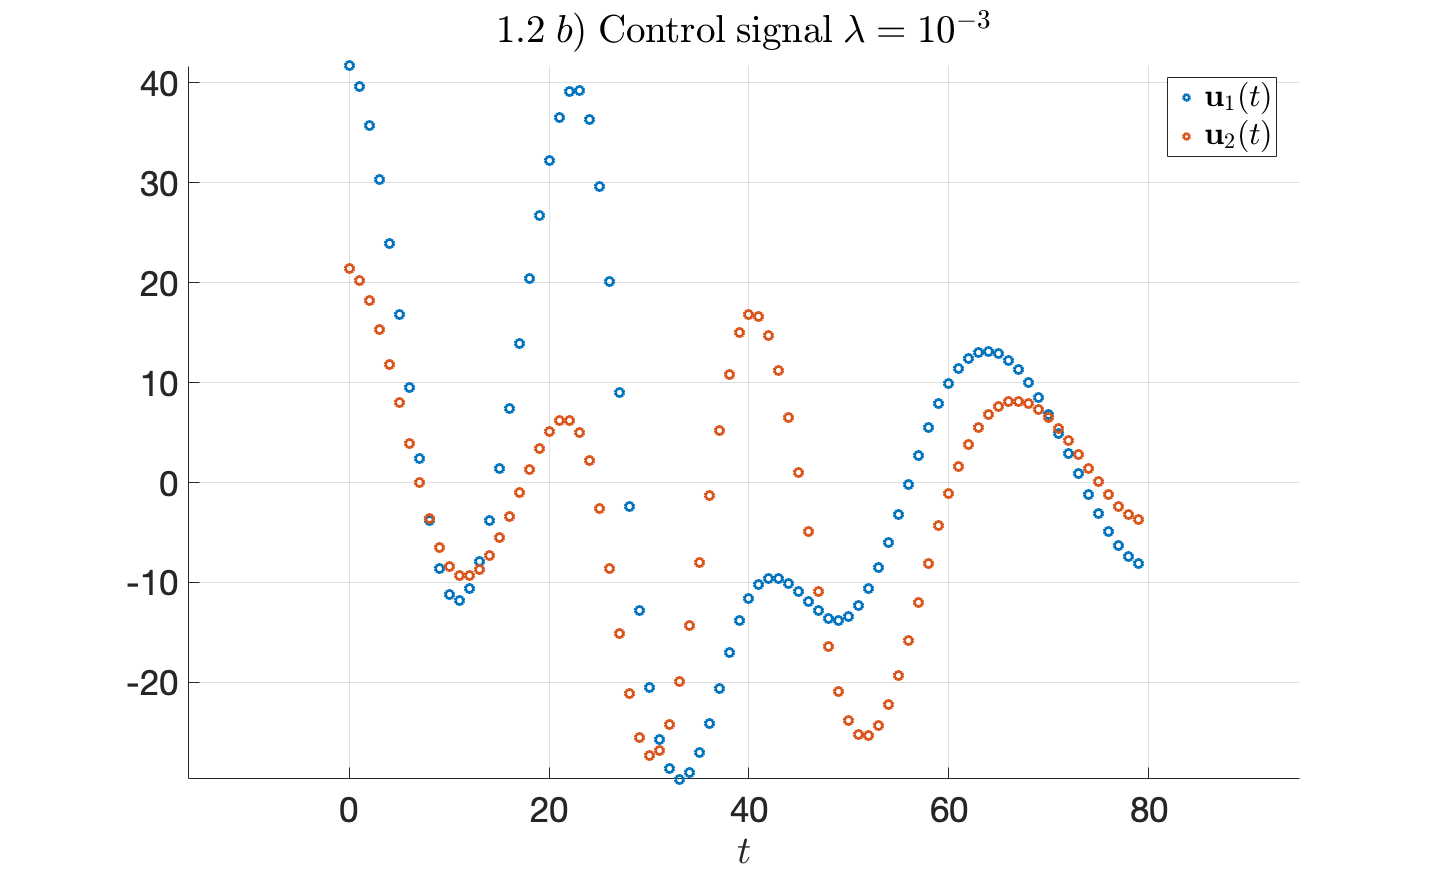
\includegraphics[width=\maxwidth{144.5057701956849em}]{figure_1}
\end{center}
\begin{matlaboutput}
1.2 c) For lambda = 1e-3 there were 79 optimal control signal changes.
1.2 d) For lambda = 1e-3 the mean deviation from the waypoints is 0.125677.
\end{matlaboutput}
\begin{center}
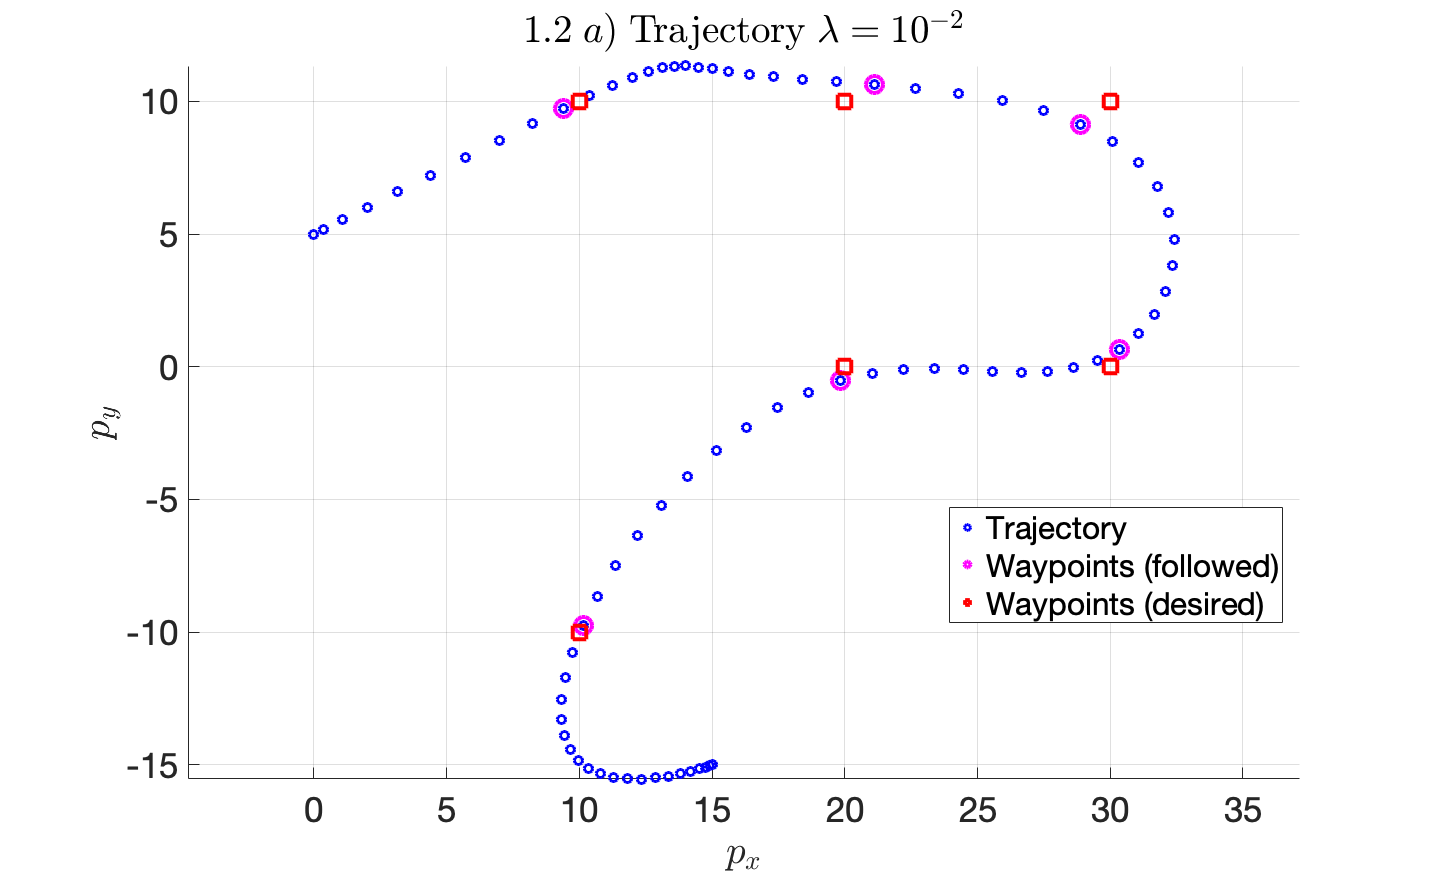
\includegraphics[width=\maxwidth{144.5057701956849em}]{figure_2}
\end{center}

\begin{center}
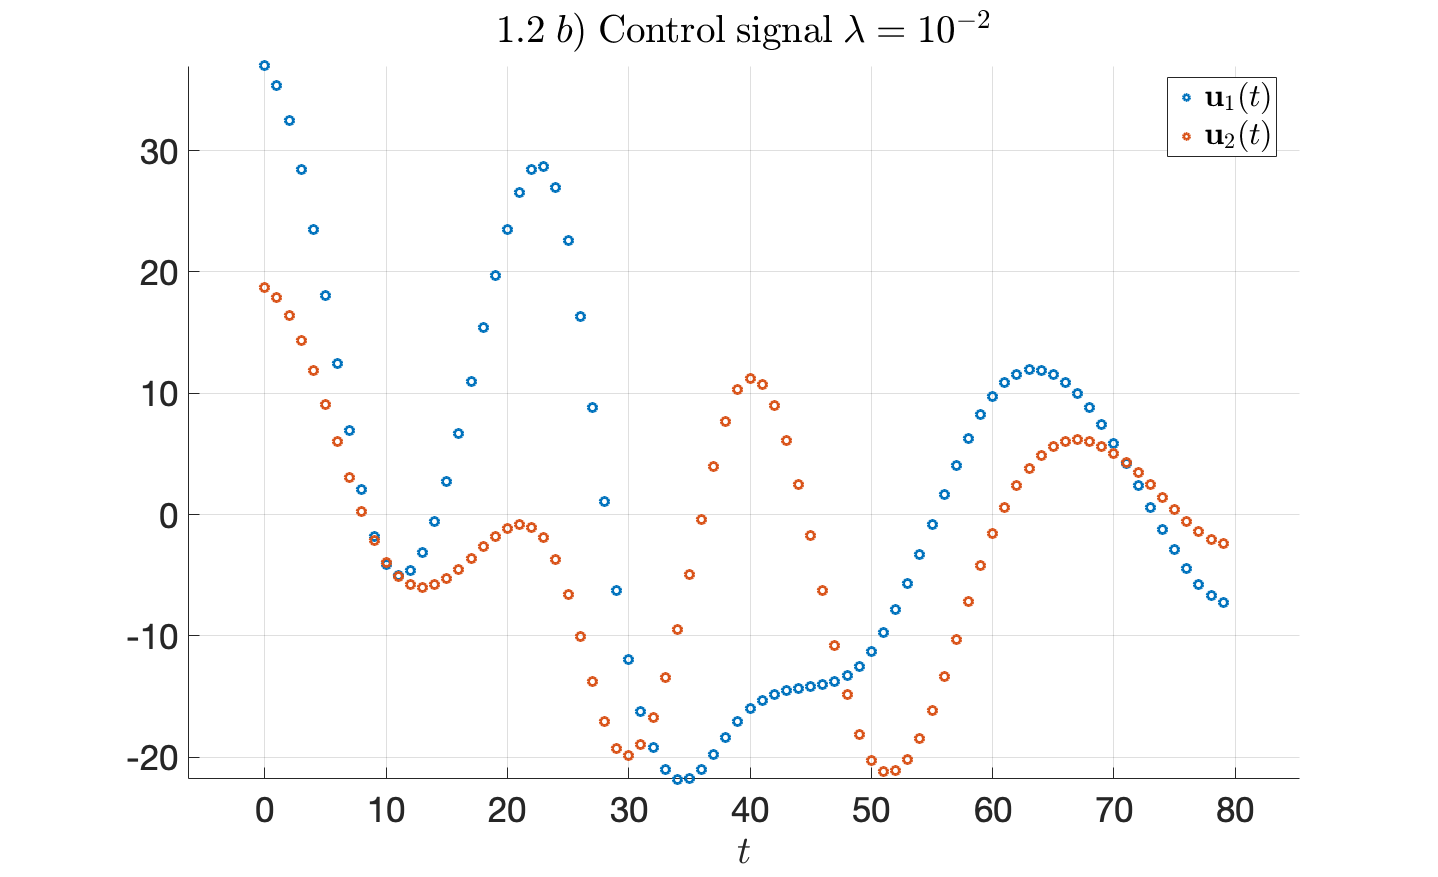
\includegraphics[width=\maxwidth{144.5057701956849em}]{figure_3}
\end{center}
\begin{matlaboutput}
1.2 c) For lambda = 1e-2 there were 79 optimal control signal changes.
1.2 d) For lambda = 1e-2 the mean deviation from the waypoints is 0.824170.
\end{matlaboutput}
\begin{center}
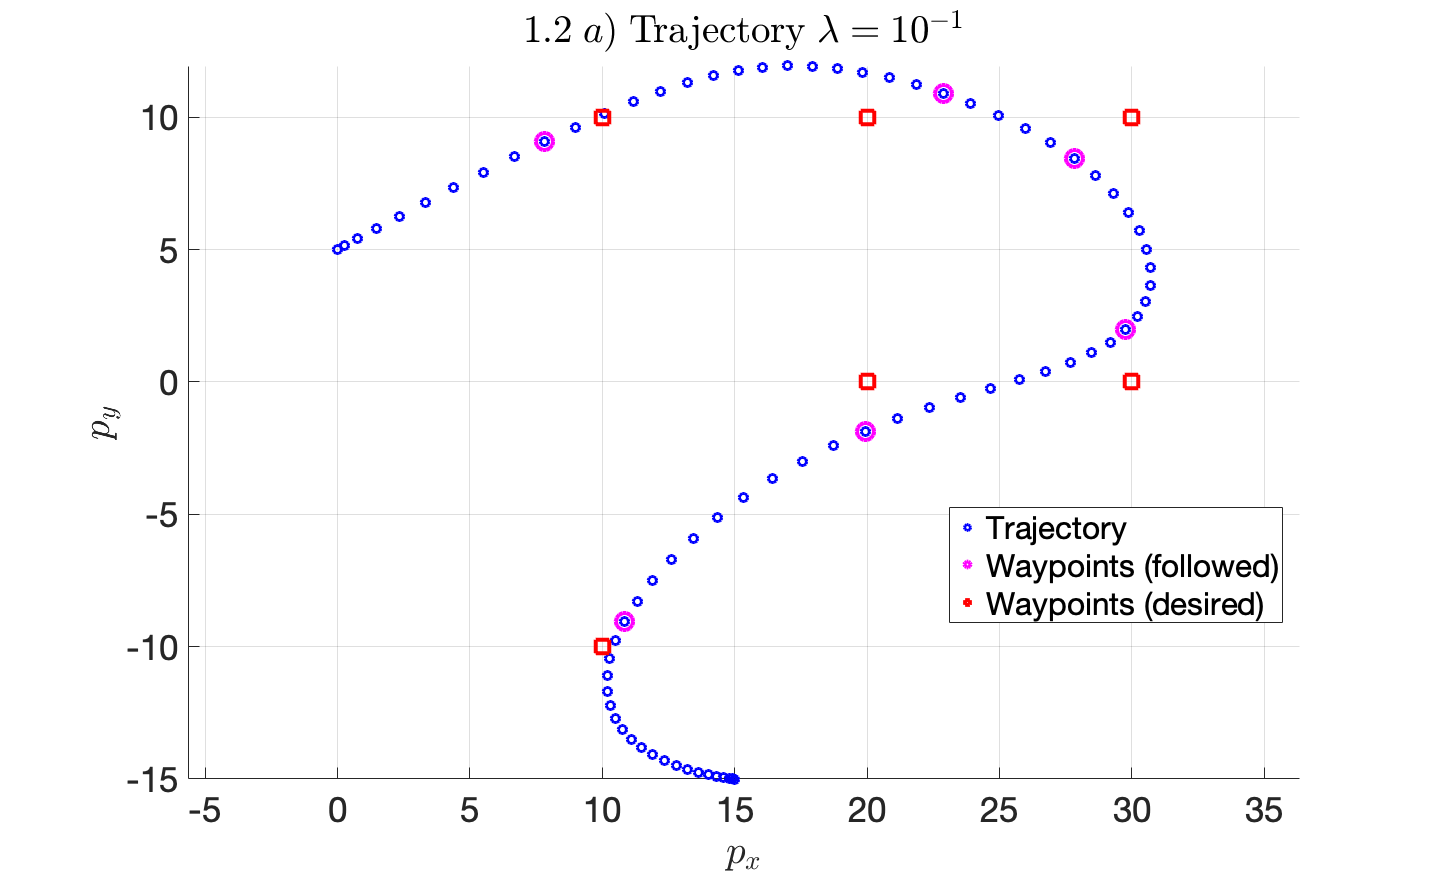
\includegraphics[width=\maxwidth{144.5057701956849em}]{figure_4}
\end{center}

\begin{center}
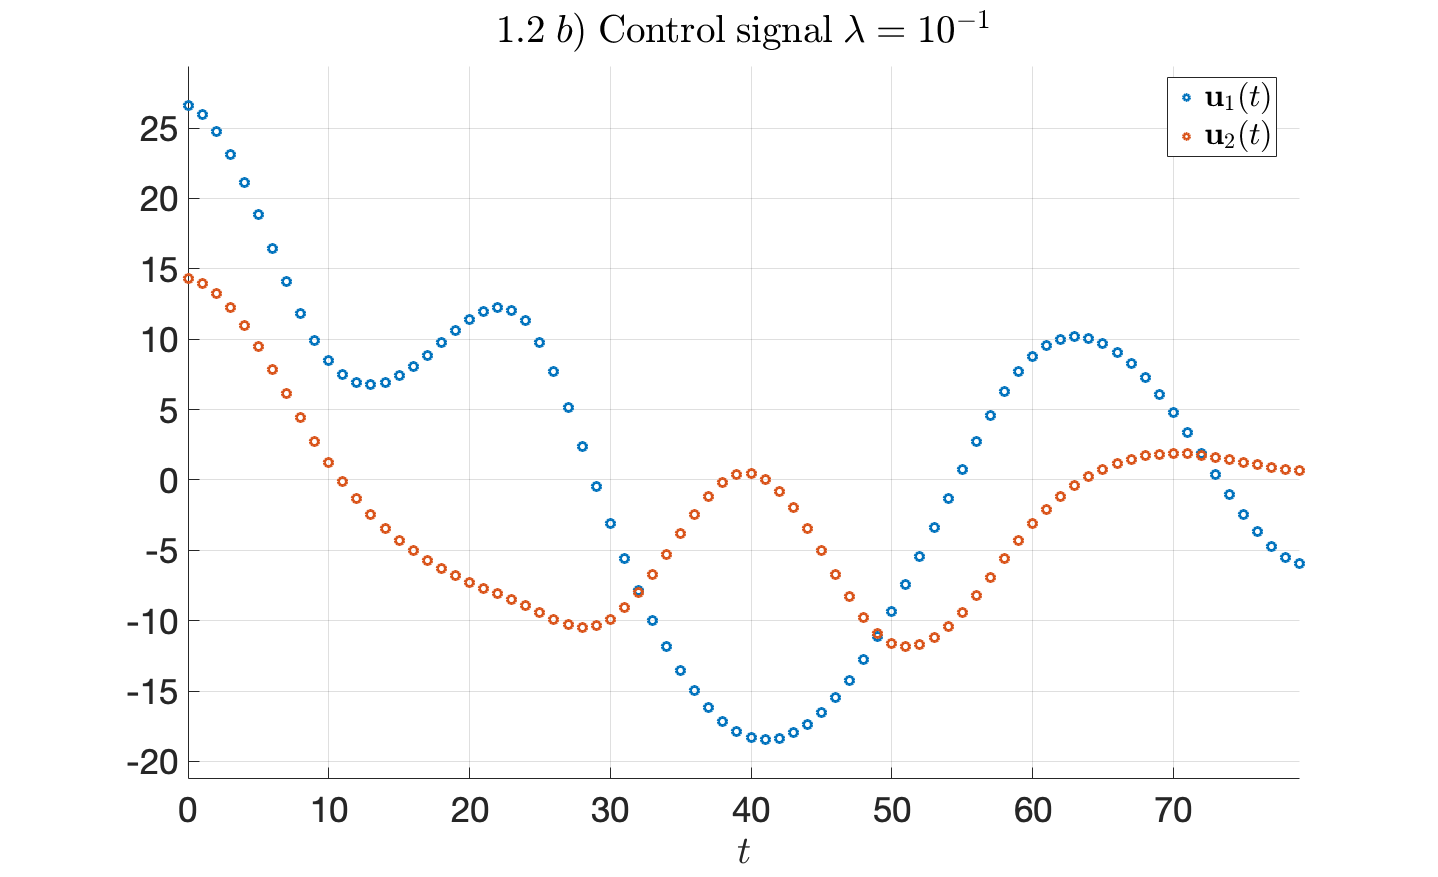
\includegraphics[width=\maxwidth{144.5057701956849em}]{figure_5}
\end{center}
\begin{matlaboutput}
1.2 c) For lambda = 1e-1 there were 79 optimal control signal changes.
1.2 d) For lambda = 1e-1 the mean deviation from the waypoints is 2.195805.
\end{matlaboutput}
\begin{center}
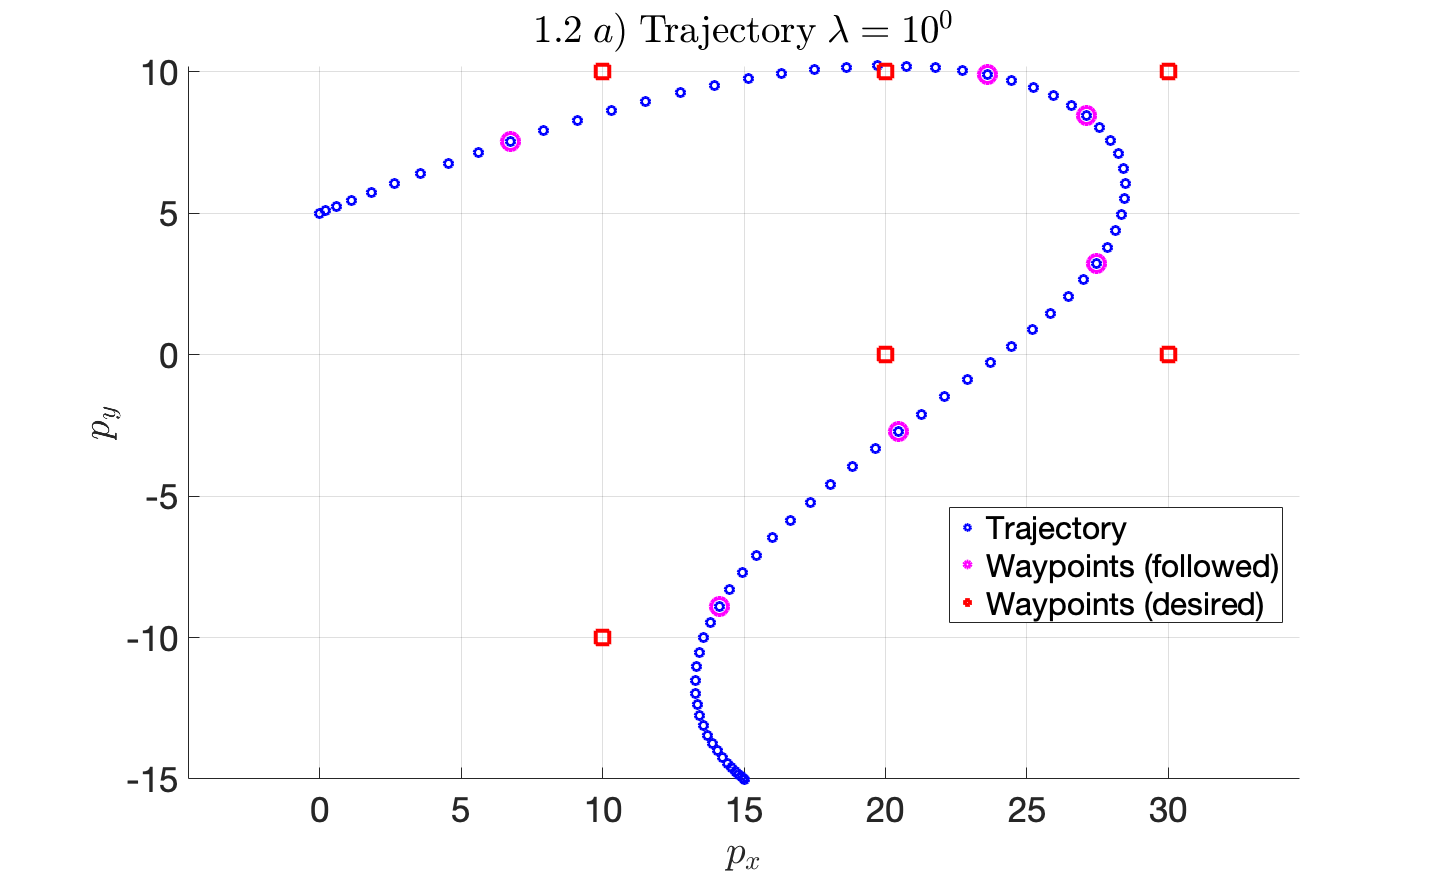
\includegraphics[width=\maxwidth{144.5057701956849em}]{figure_6}
\end{center}

\begin{center}
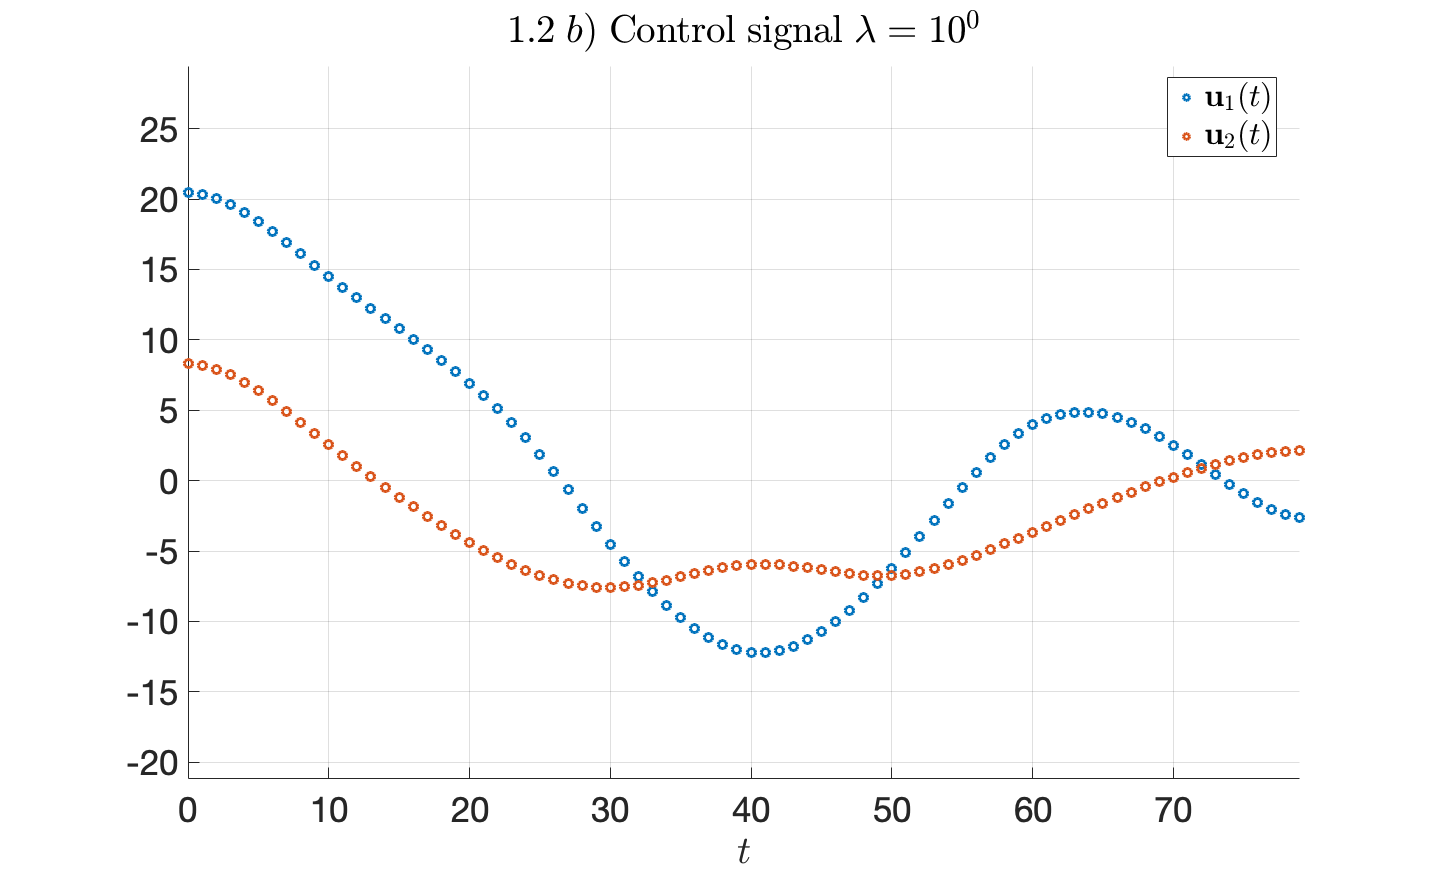
\includegraphics[width=\maxwidth{144.5057701956849em}]{figure_7}
\end{center}
\begin{matlaboutput}
1.2 c) For lambda = 1e0 there were 79 optimal control signal changes.
1.2 d) For lambda = 1e0 the mean deviation from the waypoints is 3.682588.
\end{matlaboutput}
\begin{center}
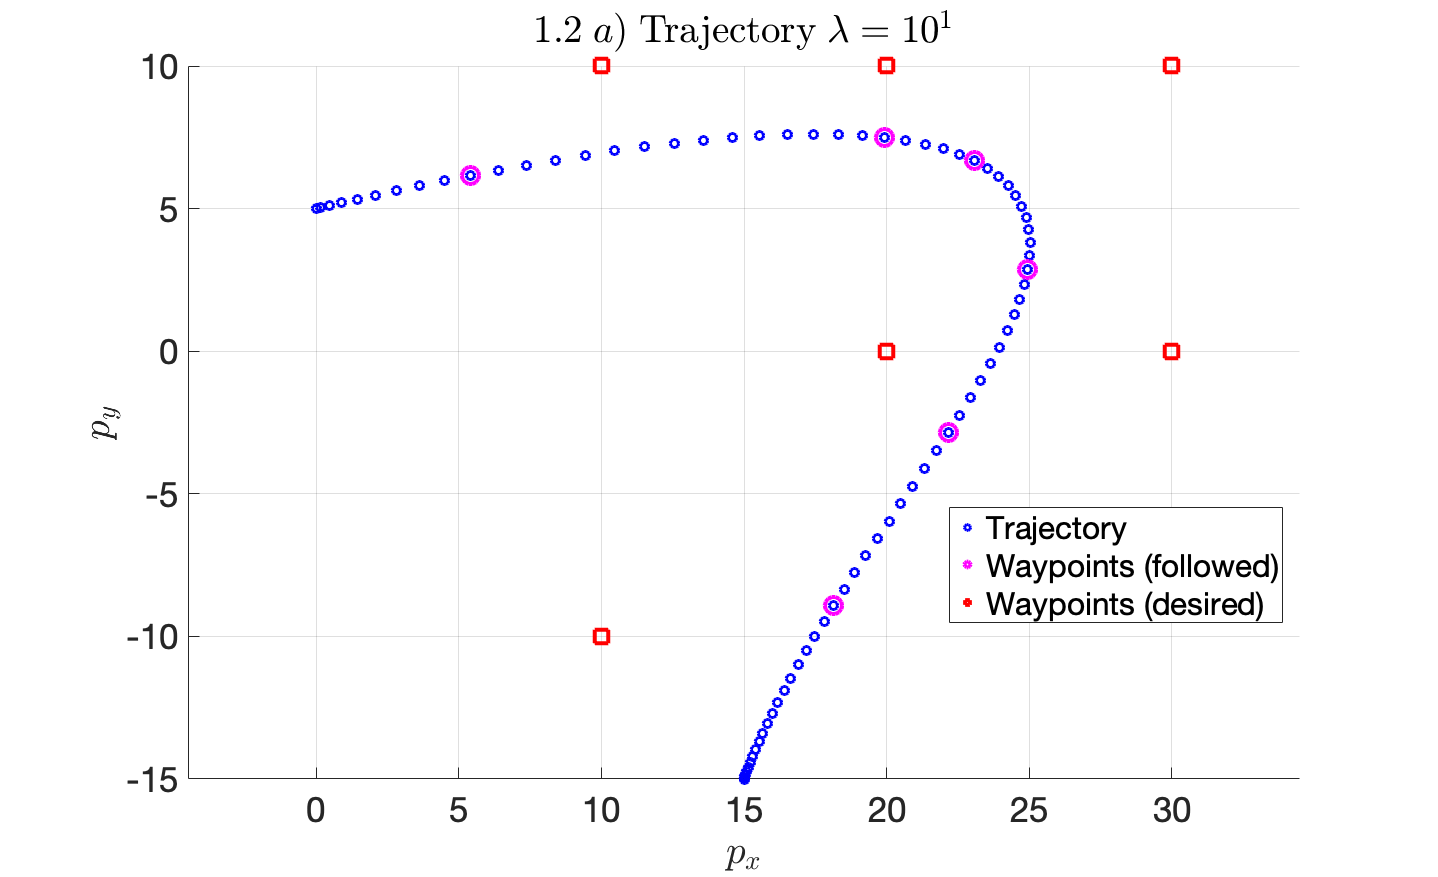
\includegraphics[width=\maxwidth{144.5057701956849em}]{figure_8}
\end{center}

\begin{center}
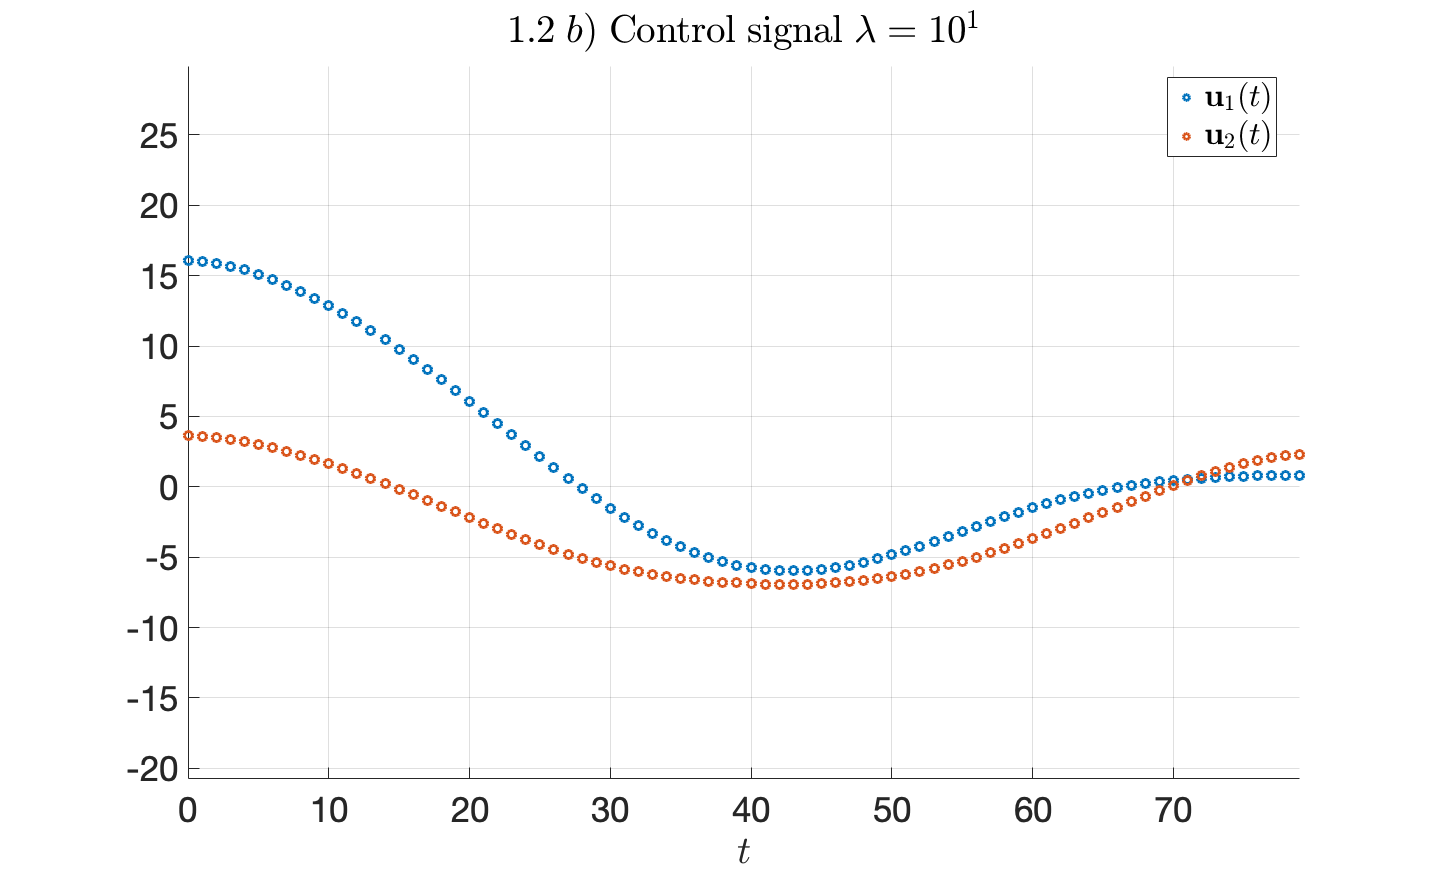
\includegraphics[width=\maxwidth{144.5057701956849em}]{figure_9}
\end{center}
\begin{matlaboutput}
1.2 c) For lambda = 1e1 there were 79 optimal control signal changes.
1.2 d) For lambda = 1e1 the mean deviation from the waypoints is 5.631691.
\end{matlaboutput}
\begin{center}
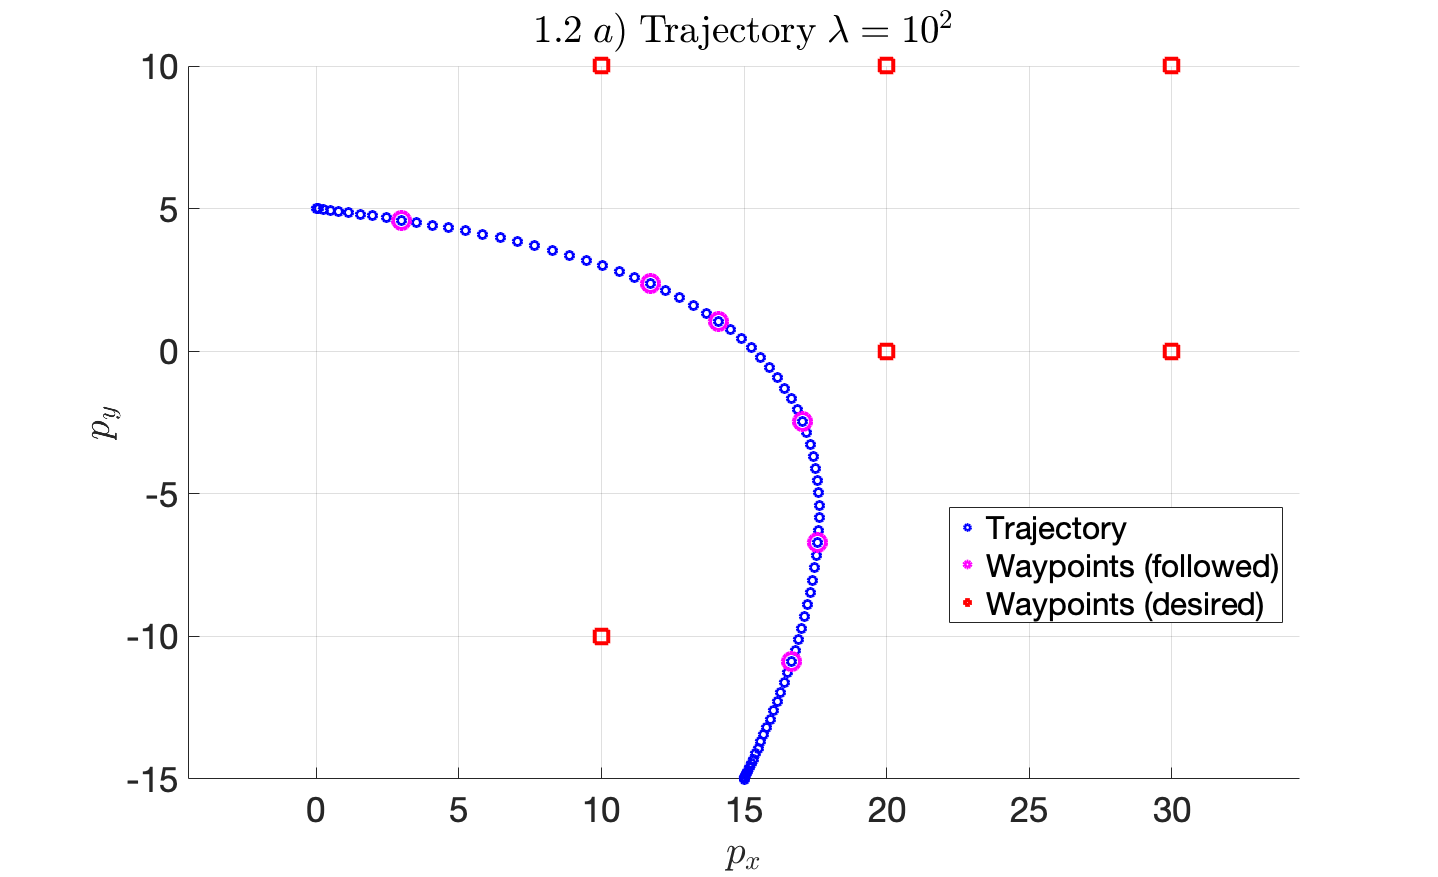
\includegraphics[width=\maxwidth{144.5057701956849em}]{figure_10}
\end{center}

\begin{center}
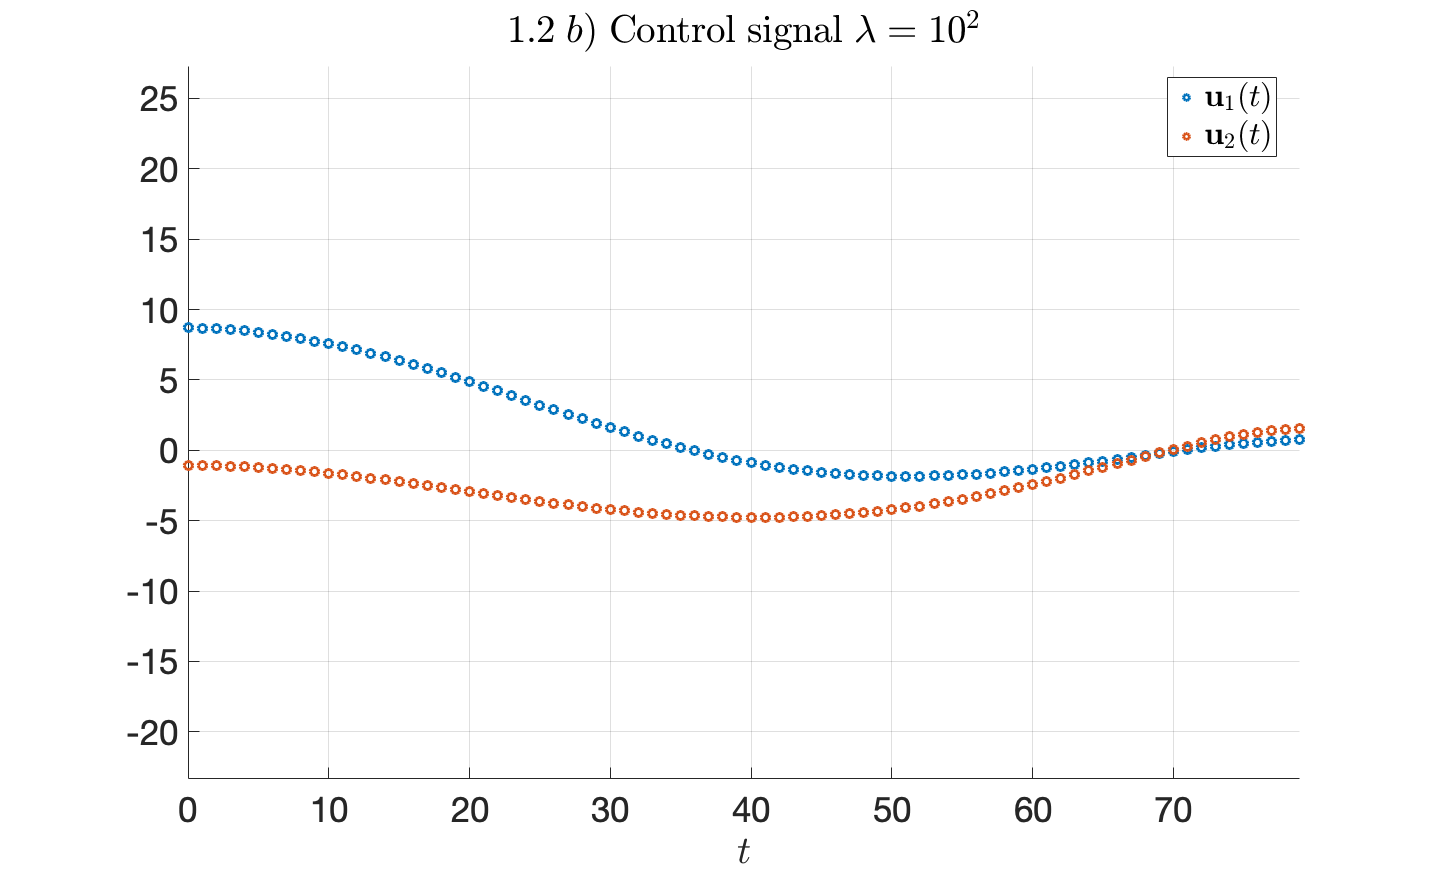
\includegraphics[width=\maxwidth{144.5057701956849em}]{figure_11}
\end{center}
\begin{matlaboutput}
1.2 c) For lambda = 1e2 there were 79 optimal control signal changes.
1.2 d) For lambda = 1e2 the mean deviation from the waypoints is 10.904150.
\end{matlaboutput}
\begin{center}
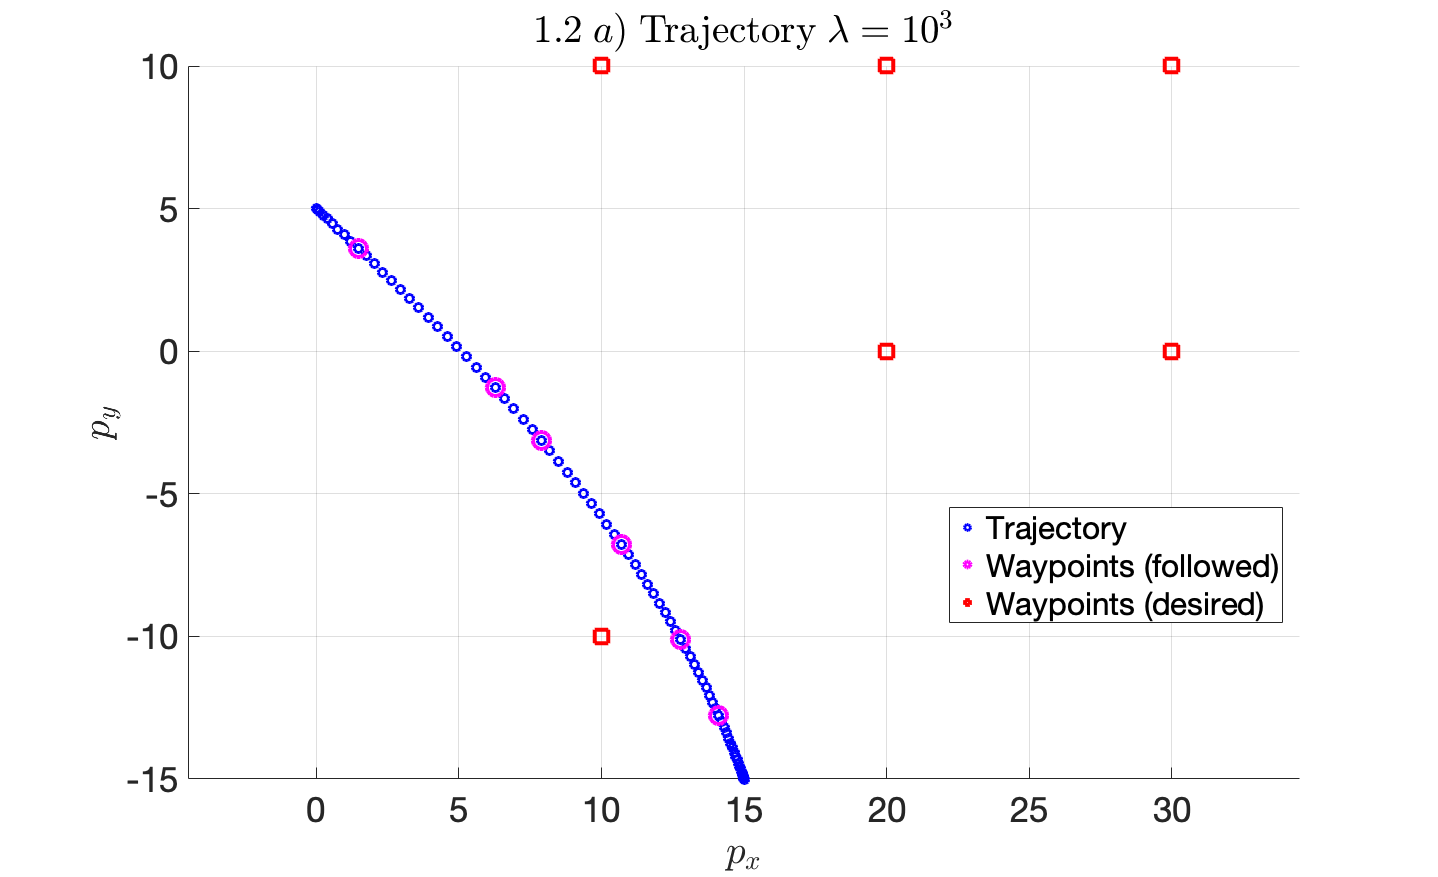
\includegraphics[width=\maxwidth{144.5057701956849em}]{figure_12}
\end{center}

\begin{center}
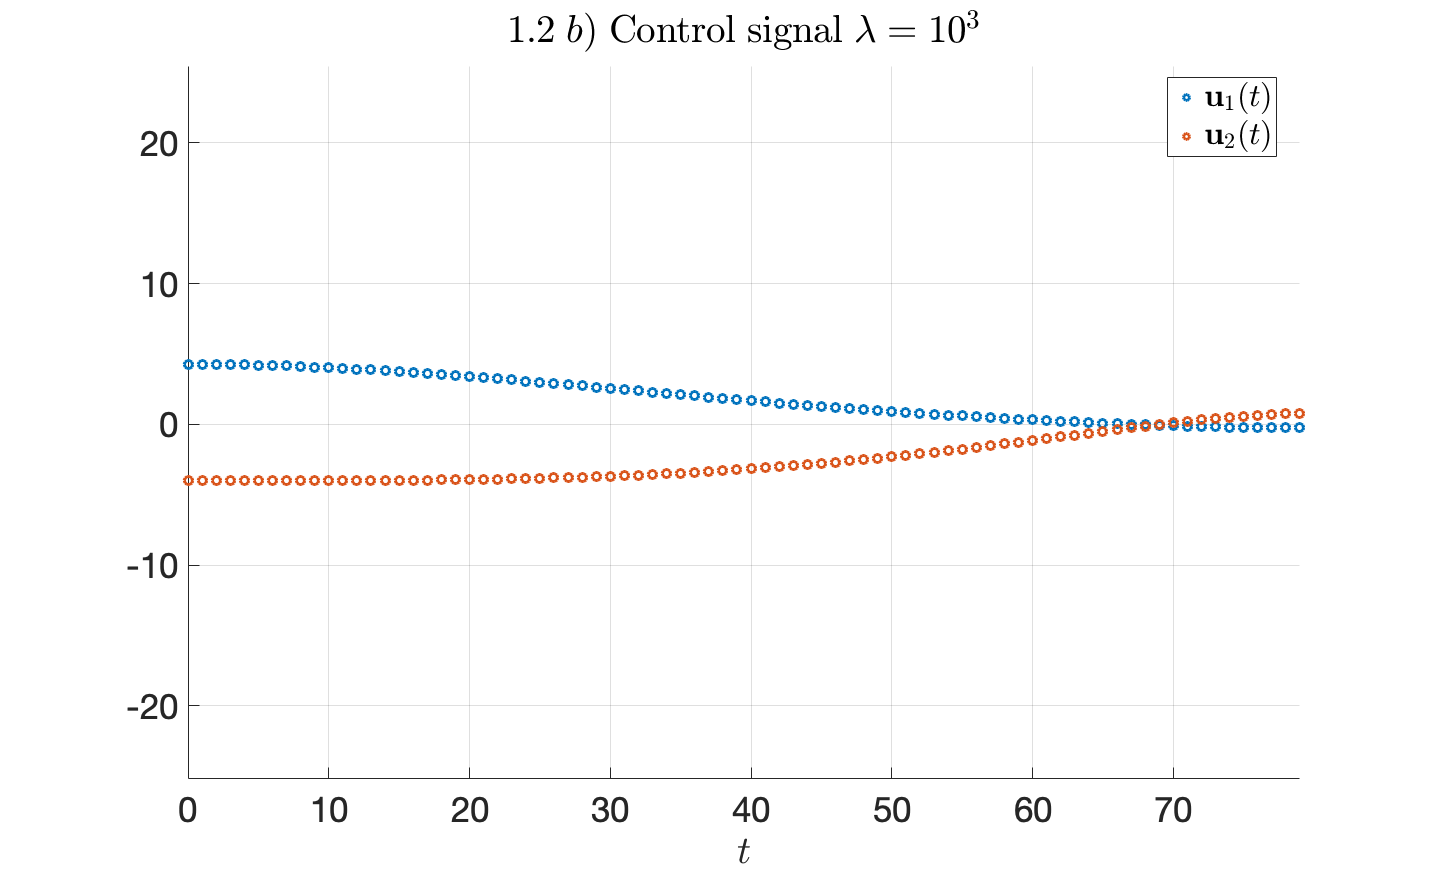
\includegraphics[width=\maxwidth{144.5057701956849em}]{figure_13}
\end{center}
\begin{matlaboutput}
1.2 c) For lambda = 1e3 there were 79 optimal control signal changes.
1.2 d) For lambda = 1e3 the mean deviation from the waypoints is 15.330435.
\end{matlaboutput}
\begin{matlabcode}
save('./transferring_a_robot_data/1_2_data_c_d.mat','controlSignalChanges','meanDeviation');

\end{matlabcode}


\matlabheading{1.3 The $l_2$ regularizer}

\begin{matlabcode}
controlSignalChanges = [];
controlSignalChangesL1 = [];
meanDeviation = [];

for lambda_log = -3:3
    % ---------- Setup optimization problem ----------
    cvx_begin quiet
        % optimization variables
        variables x(n,T+1) u(m,T)
        % cost function
        minimize(sum(sum_square(E*x(:,tau+1)-w))+...
            (10^lambda_log)*sum(norms(u*(diag(-[ones(T-1,1);0])+diag(ones(T-1,1),-1)),2)));
        % subject to
        x(:,1) == [p_initial;zeros(2,1)];
        x(:,end) == [p_final;zeros(2,1)];
        for t = 1:T
            x(:,t+1) == A*x(:,t)+B*u(:,t);
            norm(u(:,t)) <= U_max;
        end
    cvx_end
    
    % ---------- Plot result ----------
    % trajectory
    figure('units','normalized','outerposition',[0 0 1 1]);
    hold on;
    set(gca,'FontSize',35);
    ax = gca;
    ax.XGrid = 'on';
    ax.YGrid = 'on';
    axis equal;
    title(strcat('$1.3\;a)\; \mathrm{Trajectory}\;\lambda =',sprintf('10^{%d}$',lambda_log)),'Interpreter','latex');
    scatter(x(1,:),x(2,:),70,'o','blue','LineWidth',3);
    scatter(x(1,tau+1),x(2,tau+1),300,'o','magenta','LineWidth',4);
    scatter(w(1,:),w(2,:),300,'s','red','LineWidth',4);
    legend('Trajectory','Waypoints (followed)', 'Waypoints (desired)','Location','best');
    ylabel('$p_y$','Interpreter','latex');
    xlabel('$p_x$','Interpreter','latex');
    saveas(gcf,sprintf('./transferring_a_robot_data/1_3_trajectory_1e%d.fig',lambda_log));
    saveas(gcf,sprintf('./transferring_a_robot_data/1_3_trajectory_1e%d.png',lambda_log));
    hold off; 
    
    % control signal
    figure('units','normalized','outerposition',[0 0 1 1]);
    hold on;
    set(gca,'FontSize',35);
    ax = gca;
    ax.XGrid = 'on';
    ax.YGrid = 'on';
    axis equal;
    title(strcat('$1.3\;b)\; \mathrm{Control}\;\mathrm{signal}\;\lambda =',sprintf('10^{%d}$',lambda_log)),'Interpreter','latex');
    scatter(0:T-1,u(1,:),70,'o','LineWidth',3);
    scatter(0:T-1,u(2,:),70,'o','LineWidth',3);
    legend({'$\mathbf{u}_1(t)$','$\mathbf{u}_2(t)$'},'Location','best','interpreter','latex');
    ylabel('$ $','Interpreter','latex');
    xlabel('$t$','Interpreter','latex');
    saveas(gcf,sprintf('./transferring_a_robot_data/1_3_controlSignal_1e%d.fig',lambda_log));
    saveas(gcf,sprintf('./transferring_a_robot_data/1_3_controlSignal_1e%d.png',lambda_log));
    hold off;
    
    controlSignalChangesCur = 0;
    for t = 1:T-1
        if norm(u(:,t+1)-u(:,t))>1e-4
            controlSignalChangesCur = controlSignalChangesCur+1;
        end
    end
    controlSignalChanges = [controlSignalChanges [10^lambda_log;controlSignalChangesCur]]; 
    fprintf("1.3 c) For lambda = 1e%d there were %d optimal control signal changes.\n",lambda_log,controlSignalChangesCur);
    
    controlSignalChangesCurL1 = 0;
    for t = 1:T-1
        if norms(u(:,t+1)-u(:,t),1)>1e-4
            controlSignalChangesCurL1 = controlSignalChangesCurL1+1;
        end
    end
    controlSignalChangesL1 = [controlSignalChangesL1 [10^lambda_log;controlSignalChangesCurL1]]; 
    fprintf("1.3 c) For lambda = 1e%d there were %d optimal control signal L1 changes.\n",lambda_log,controlSignalChangesCurL1);
    
    meanDeviationCur = (1/length(w))*sum(sqrt(sum_square(E*x(:,tau+1)-w)));
    meanDeviation = [meanDeviation [10^lambda_log; meanDeviationCur]];
    fprintf("1.3 d) For lambda = 1e%d the mean deviation from the waypoints is %f.\n",lambda_log,meanDeviationCur);
end
\end{matlabcode}
\begin{center}
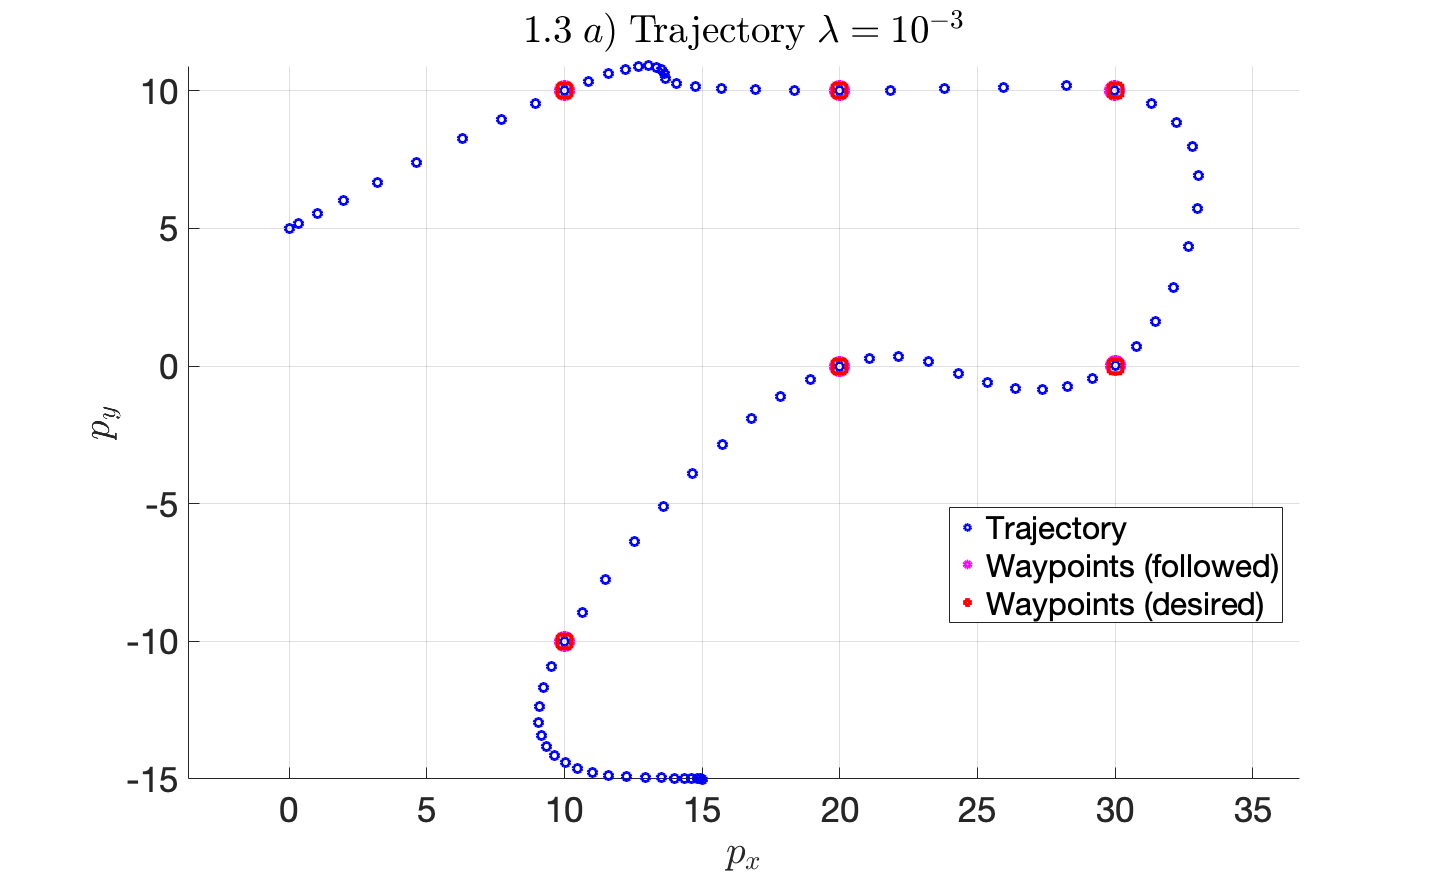
\includegraphics[width=\maxwidth{144.5057701956849em}]{figure_14}
\end{center}

\begin{center}
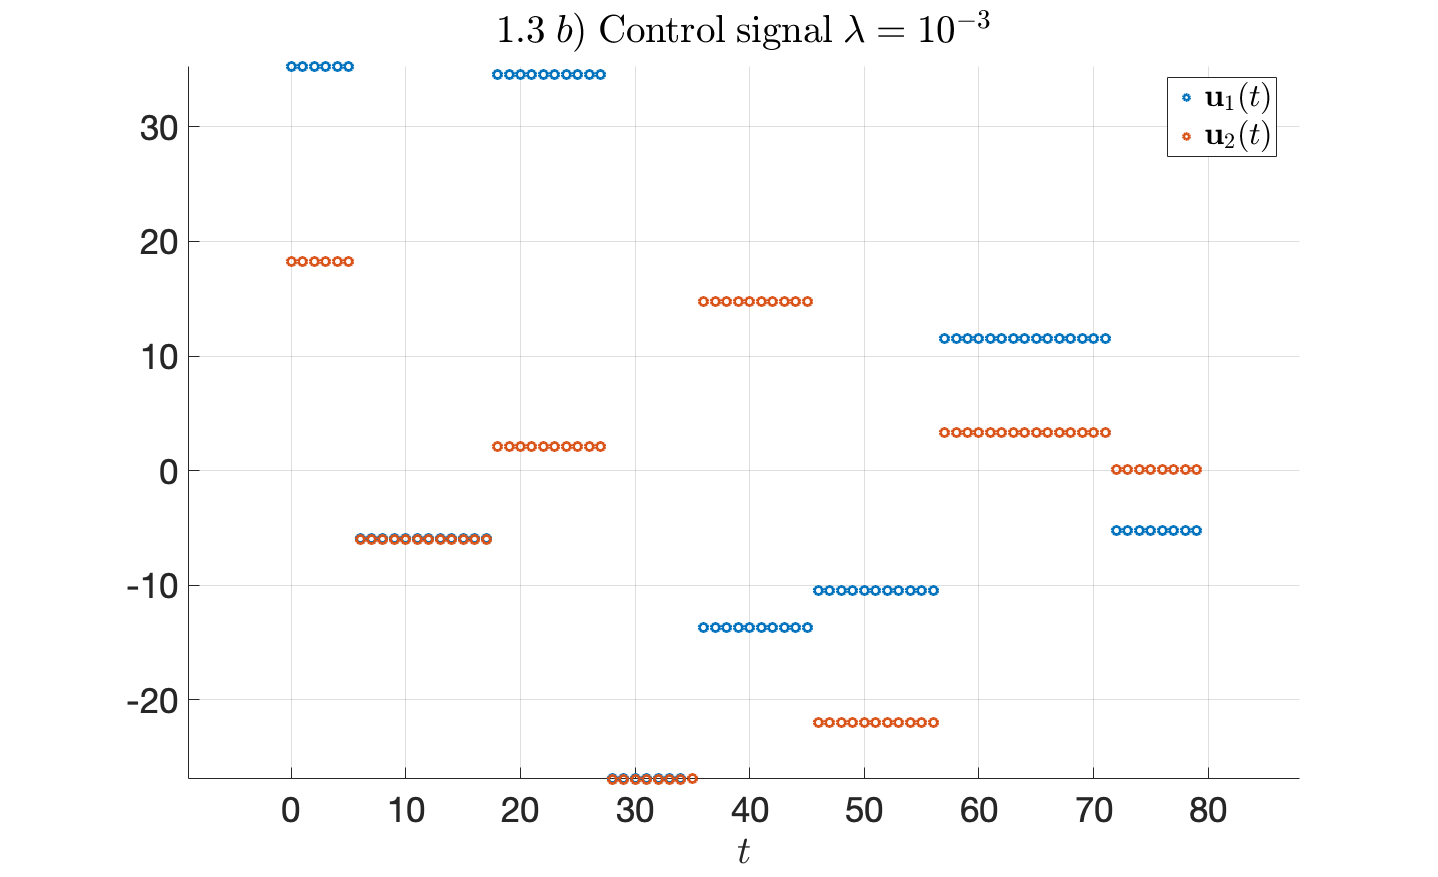
\includegraphics[width=\maxwidth{144.5057701956849em}]{figure_15}
\end{center}
\begin{matlaboutput}
1.3 c) For lambda = 1e-3 there were 7 optimal control signal changes.
1.3 c) For lambda = 1e-3 there were 7 optimal control signal L1 changes.
1.3 d) For lambda = 1e-3 the mean deviation from the waypoints is 0.007501.
\end{matlaboutput}
\begin{center}
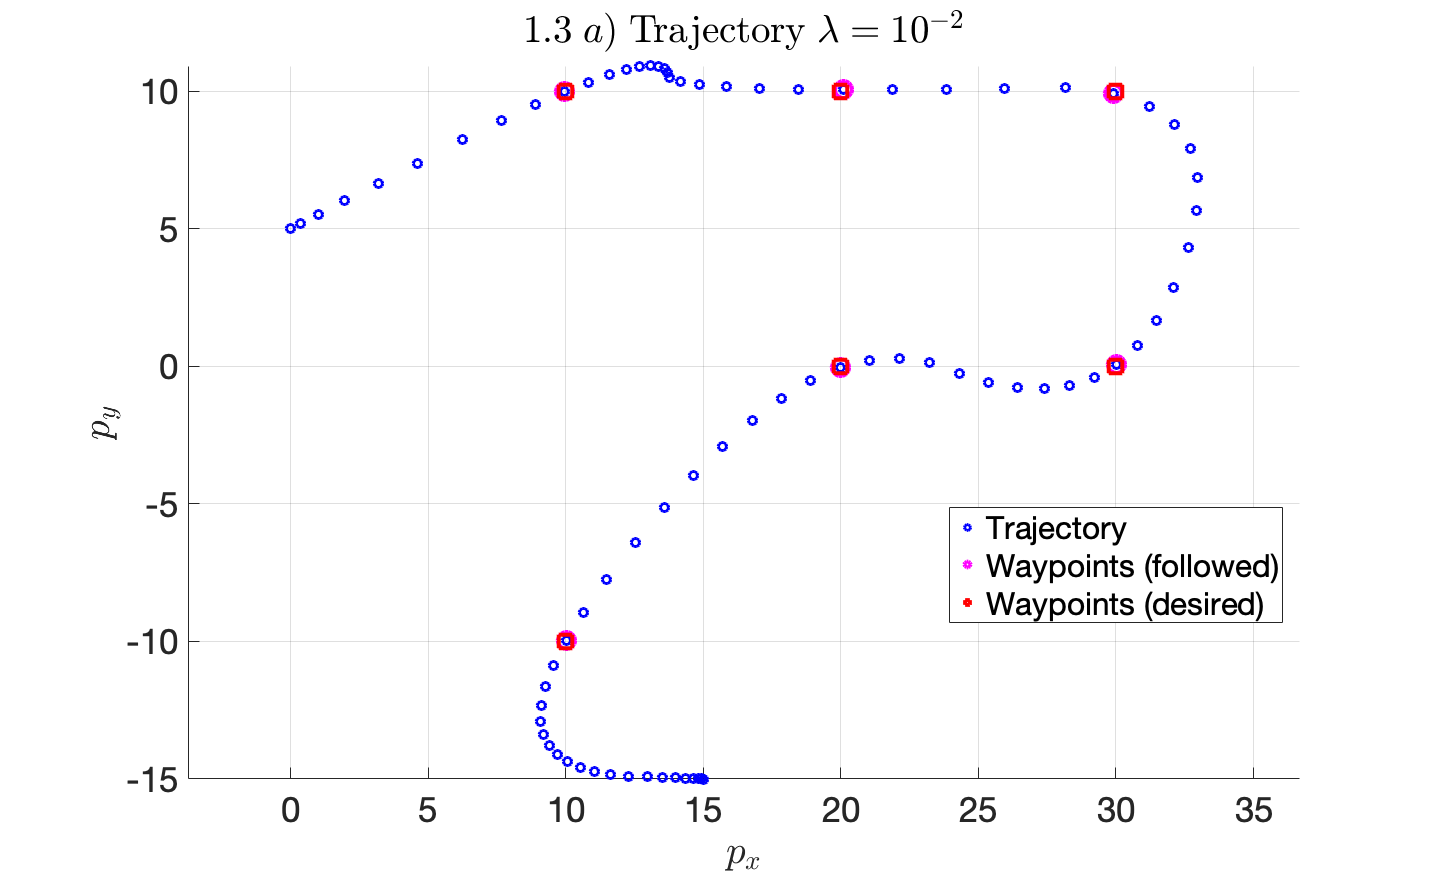
\includegraphics[width=\maxwidth{144.5057701956849em}]{figure_16}
\end{center}

\begin{center}
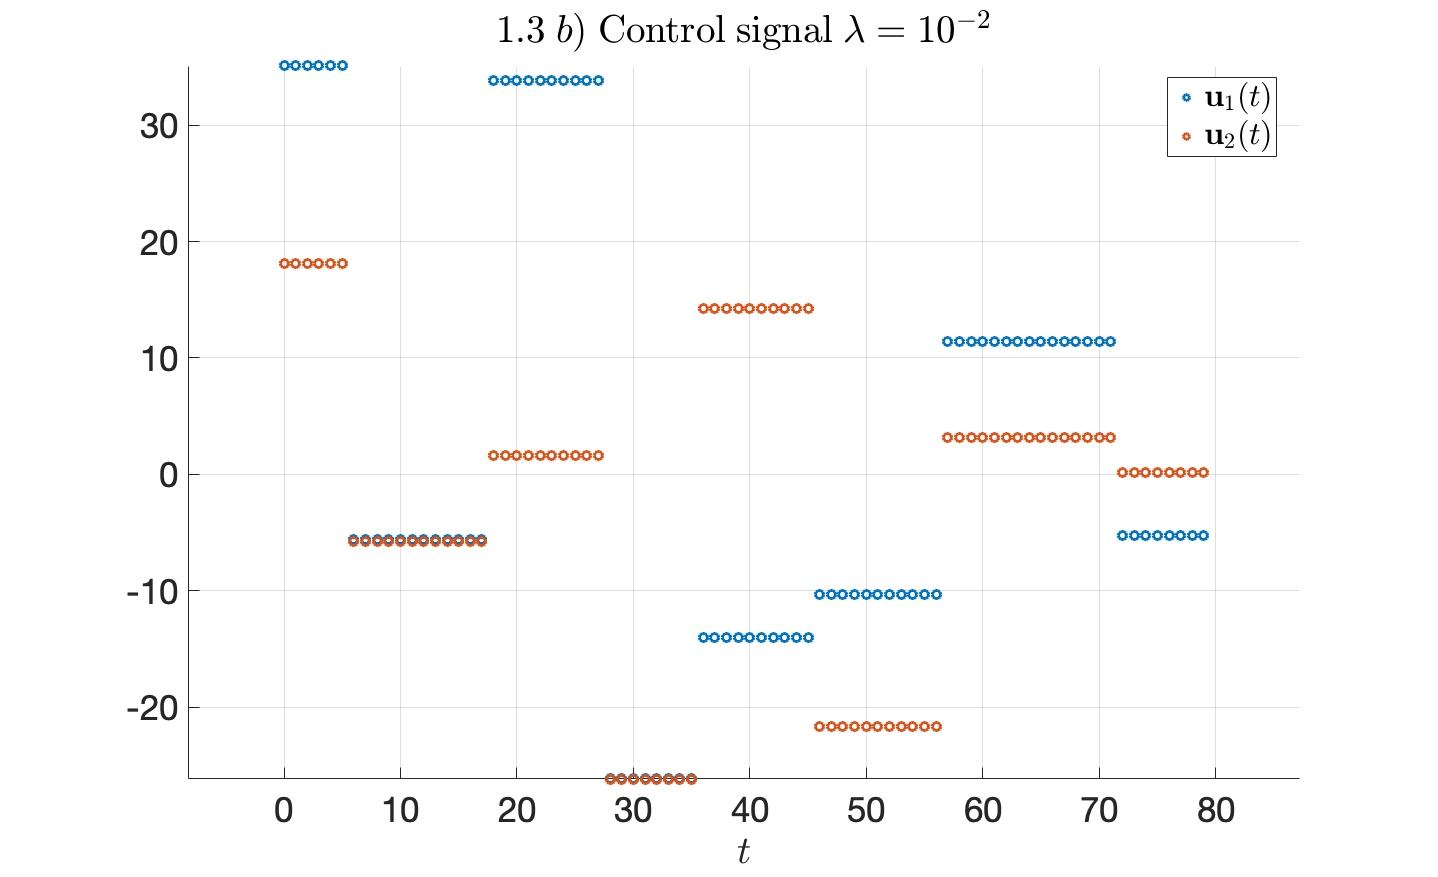
\includegraphics[width=\maxwidth{144.5057701956849em}]{figure_17}
\end{center}
\begin{matlaboutput}
1.3 c) For lambda = 1e-2 there were 7 optimal control signal changes.
1.3 c) For lambda = 1e-2 there were 7 optimal control signal L1 changes.
1.3 d) For lambda = 1e-2 the mean deviation from the waypoints is 0.074656.
\end{matlaboutput}
\begin{center}
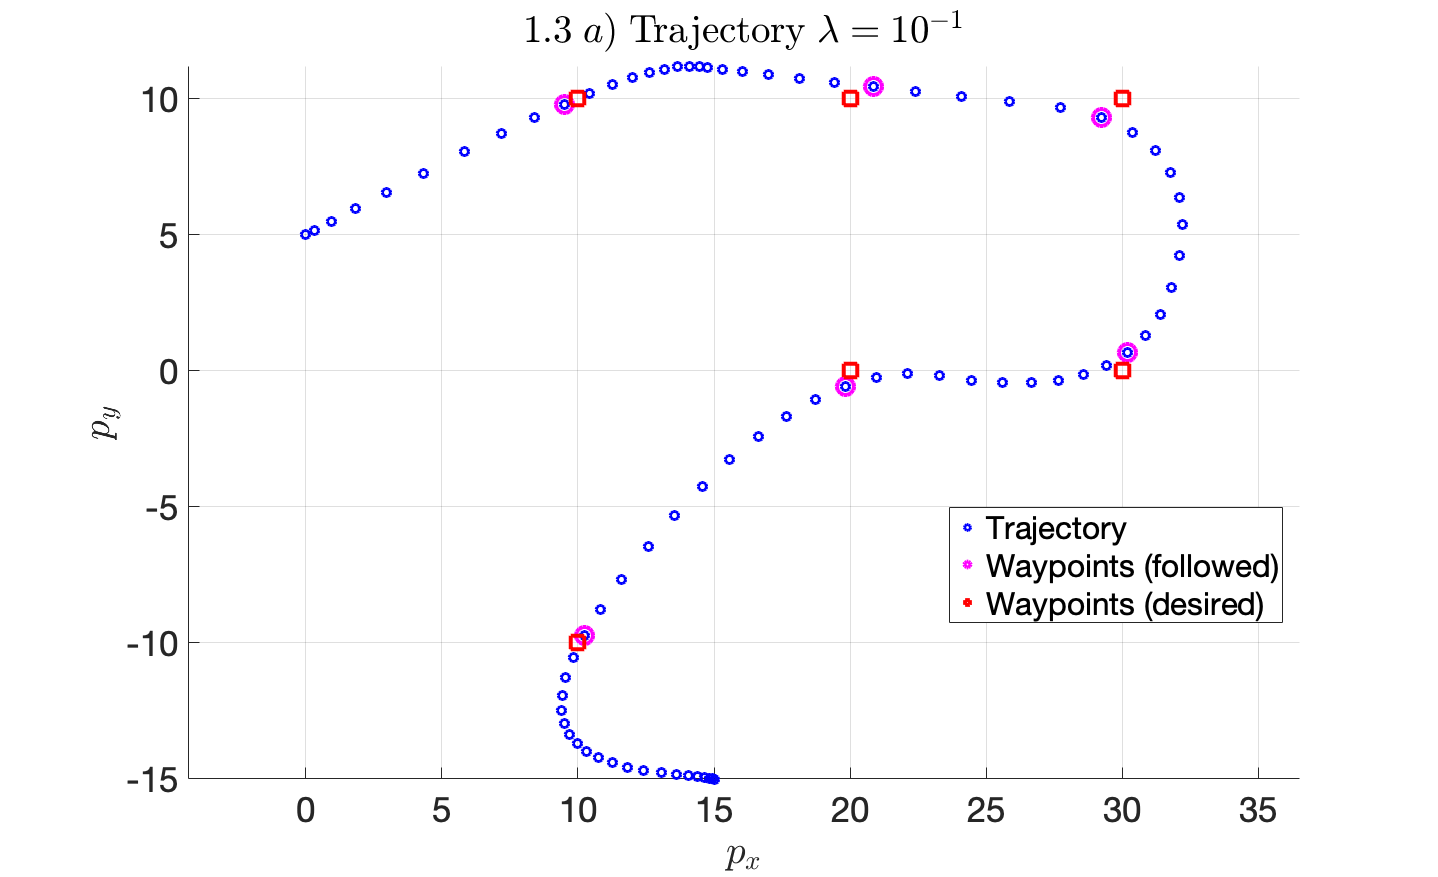
\includegraphics[width=\maxwidth{144.5057701956849em}]{figure_18}
\end{center}

\begin{center}
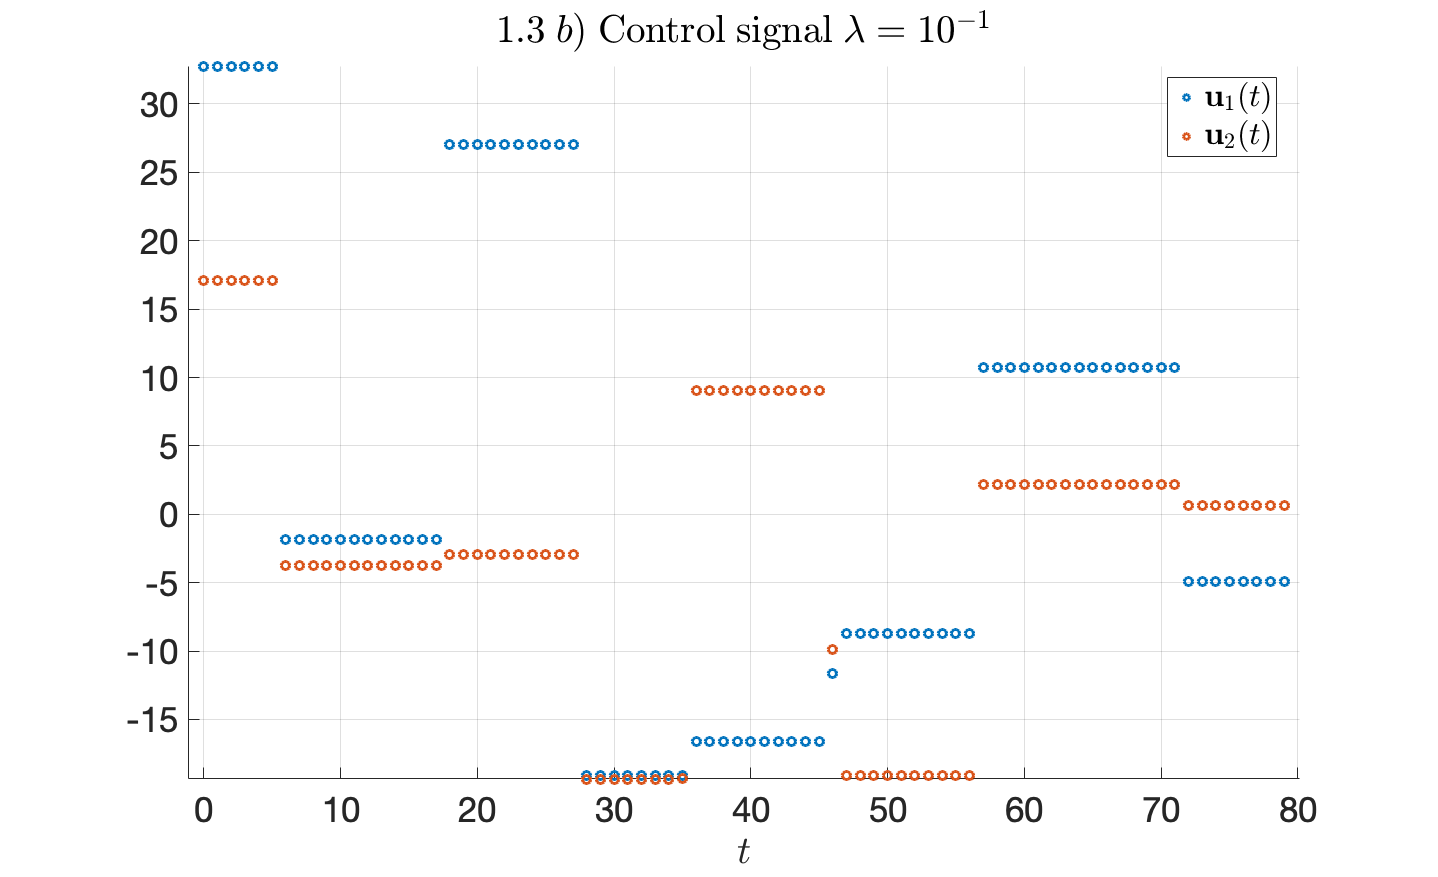
\includegraphics[width=\maxwidth{144.5057701956849em}]{figure_19}
\end{center}
\begin{matlaboutput}
1.3 c) For lambda = 1e-1 there were 8 optimal control signal changes.
1.3 c) For lambda = 1e-1 there were 8 optimal control signal L1 changes.
1.3 d) For lambda = 1e-1 the mean deviation from the waypoints is 0.702073.
\end{matlaboutput}
\begin{center}
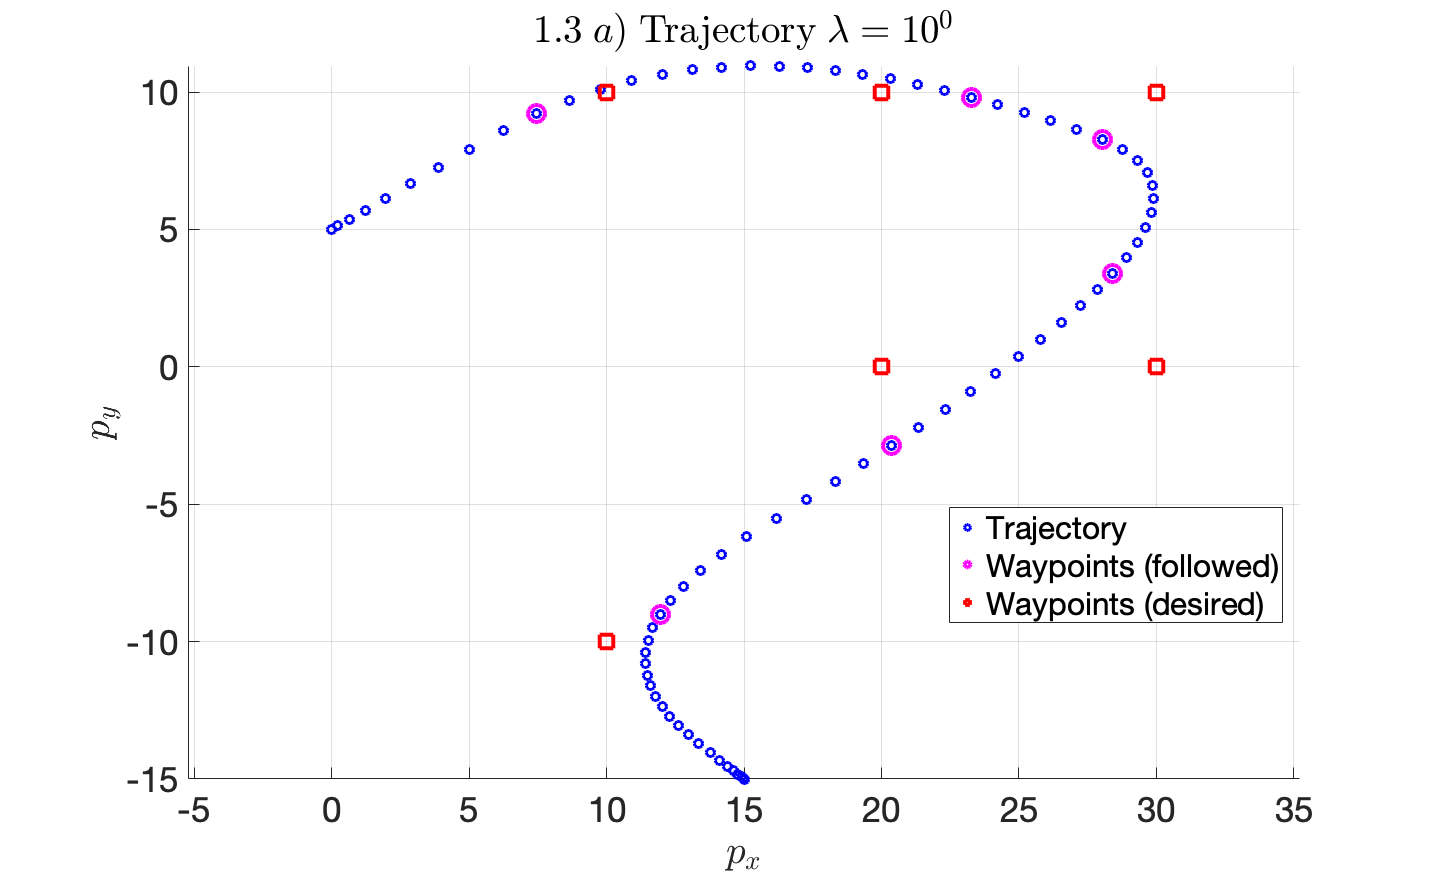
\includegraphics[width=\maxwidth{144.5057701956849em}]{figure_20}
\end{center}

\begin{center}
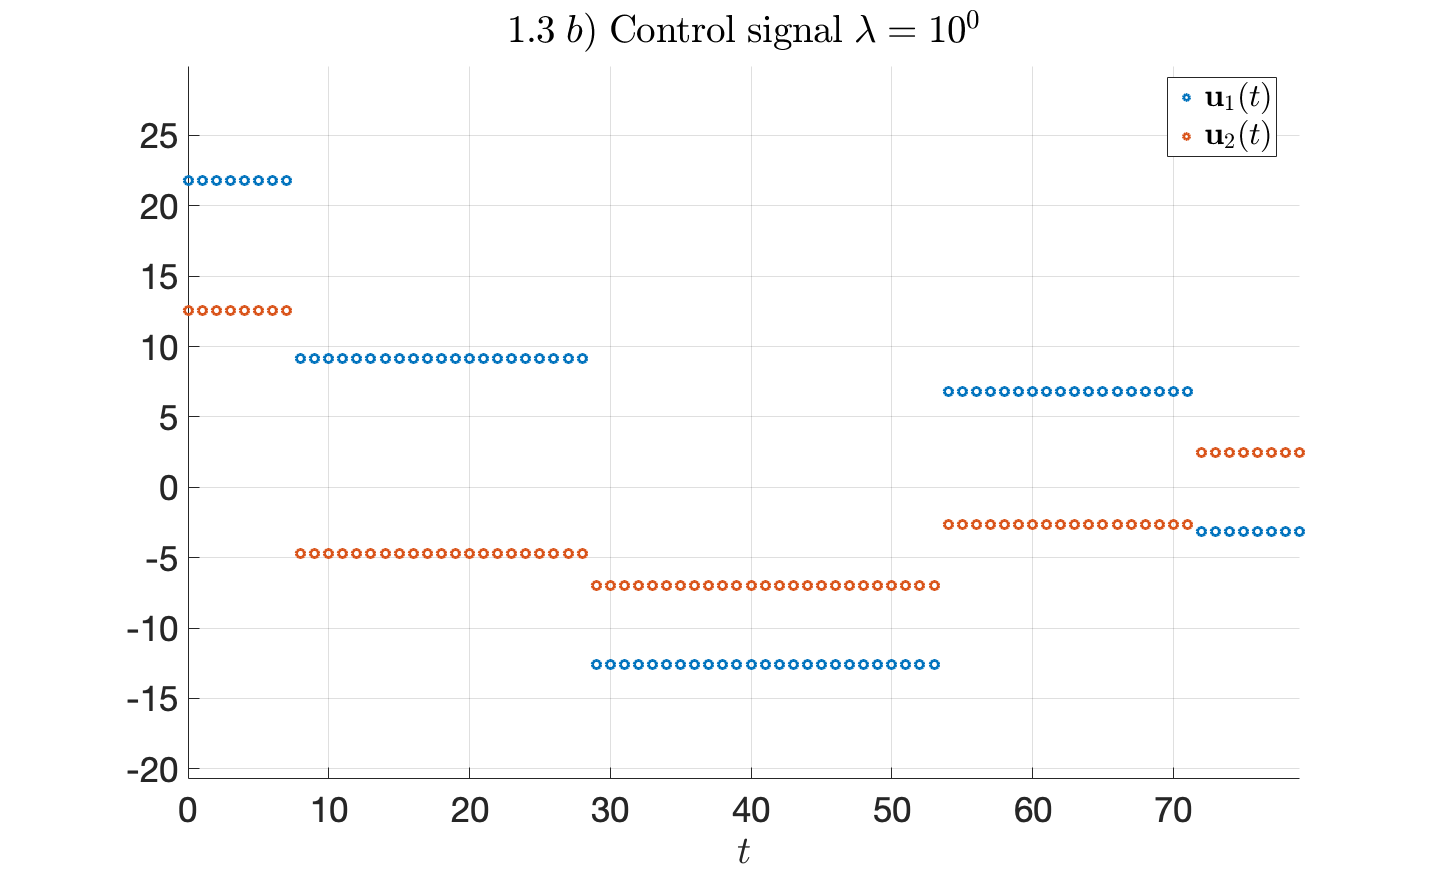
\includegraphics[width=\maxwidth{144.5057701956849em}]{figure_21}
\end{center}
\begin{matlaboutput}
1.3 c) For lambda = 1e0 there were 4 optimal control signal changes.
1.3 c) For lambda = 1e0 there were 4 optimal control signal L1 changes.
1.3 d) For lambda = 1e0 the mean deviation from the waypoints is 2.887570.
\end{matlaboutput}
\begin{center}
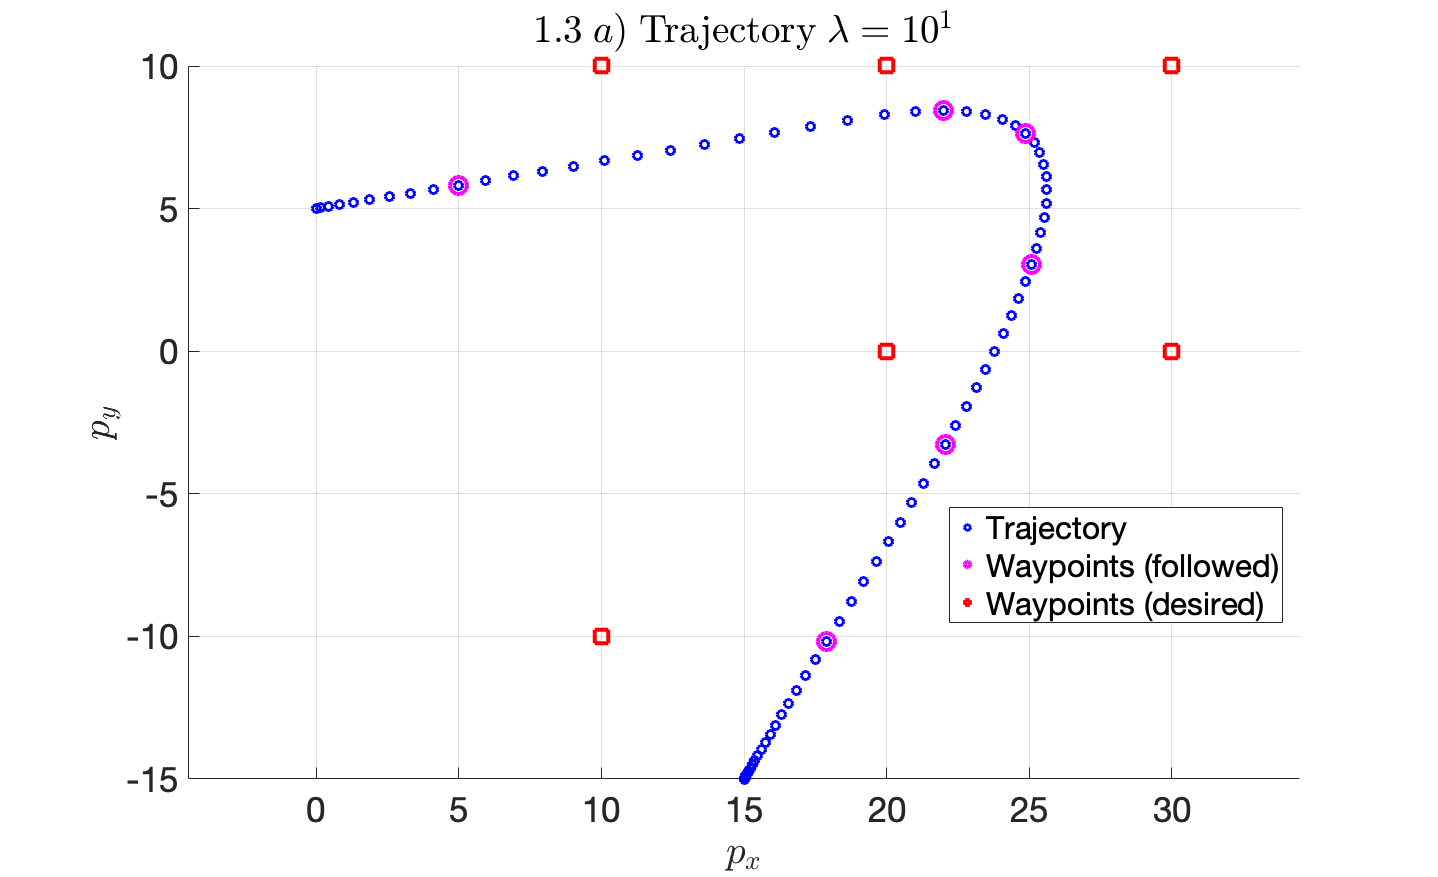
\includegraphics[width=\maxwidth{144.5057701956849em}]{figure_22}
\end{center}

\begin{center}
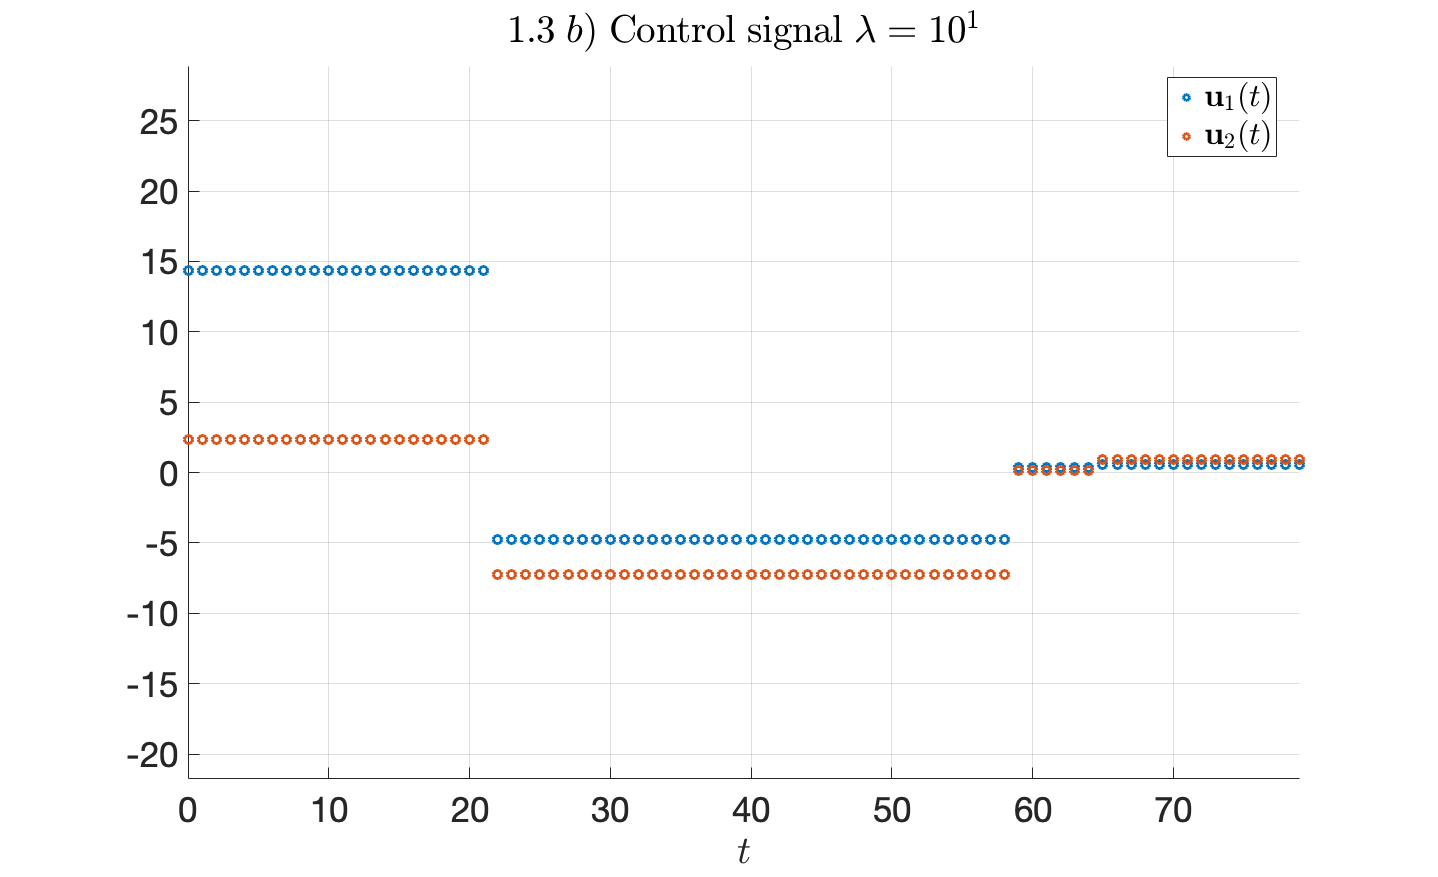
\includegraphics[width=\maxwidth{144.5057701956849em}]{figure_23}
\end{center}
\begin{matlaboutput}
1.3 c) For lambda = 1e1 there were 3 optimal control signal changes.
1.3 c) For lambda = 1e1 there were 3 optimal control signal L1 changes.
1.3 d) For lambda = 1e1 the mean deviation from the waypoints is 5.368939.
\end{matlaboutput}
\begin{center}
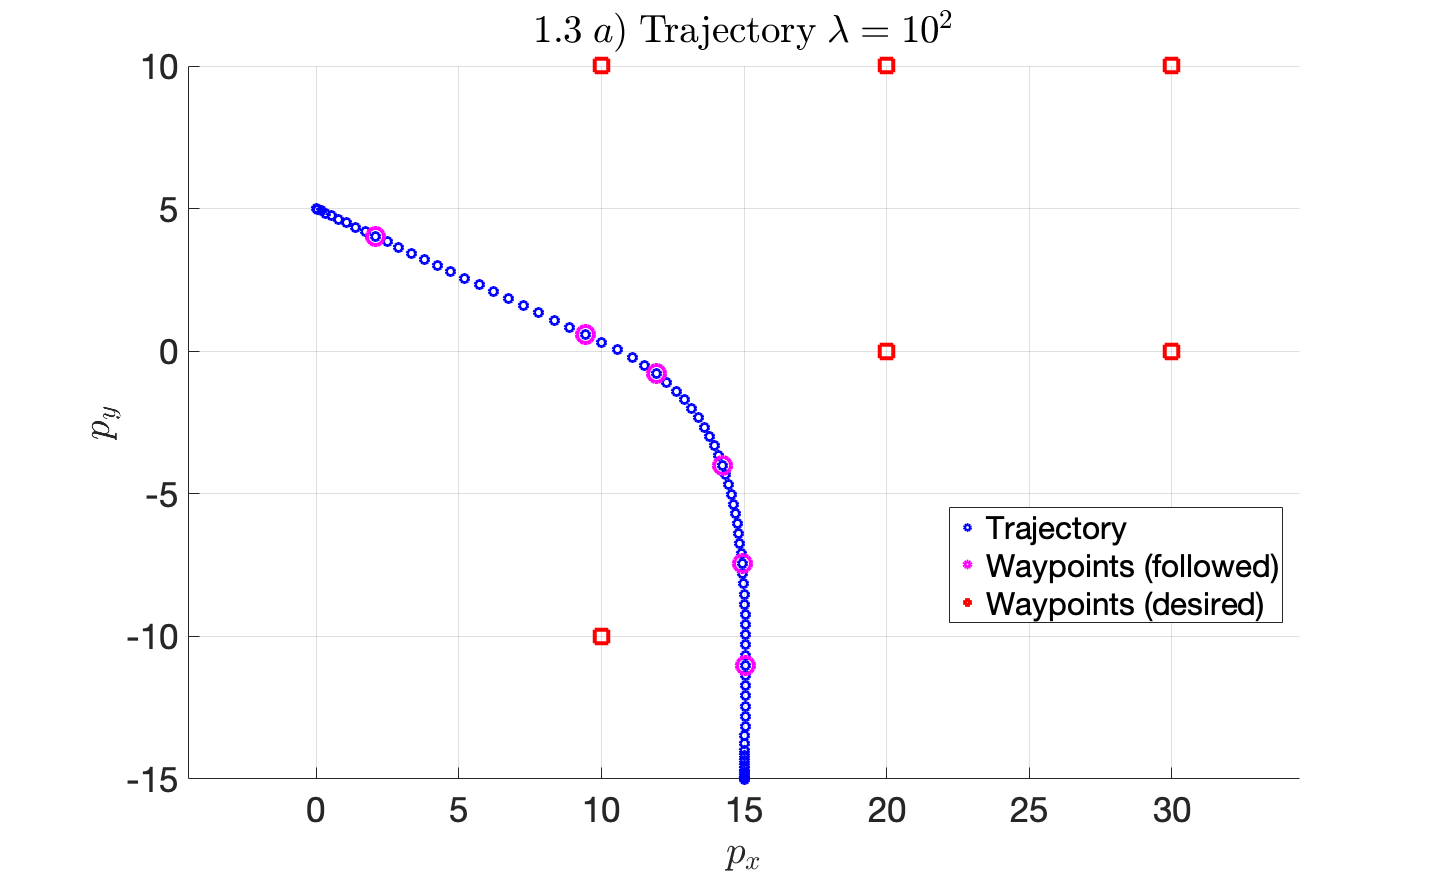
\includegraphics[width=\maxwidth{144.5057701956849em}]{figure_24}
\end{center}

\begin{center}
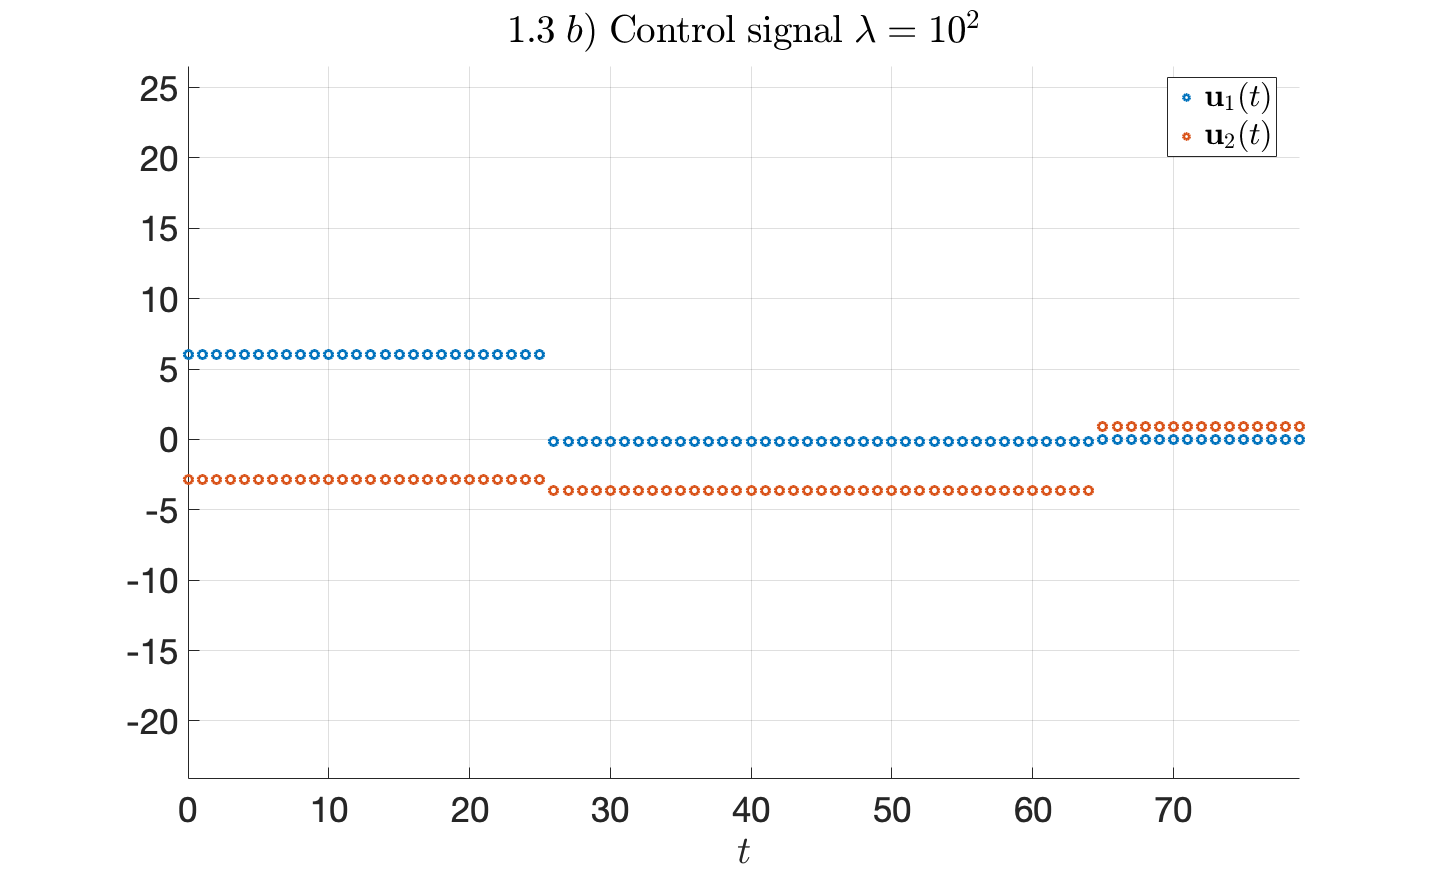
\includegraphics[width=\maxwidth{144.5057701956849em}]{figure_25}
\end{center}
\begin{matlaboutput}
1.3 c) For lambda = 1e2 there were 2 optimal control signal changes.
1.3 c) For lambda = 1e2 there were 2 optimal control signal L1 changes.
1.3 d) For lambda = 1e2 the mean deviation from the waypoints is 12.591431.
\end{matlaboutput}
\begin{center}
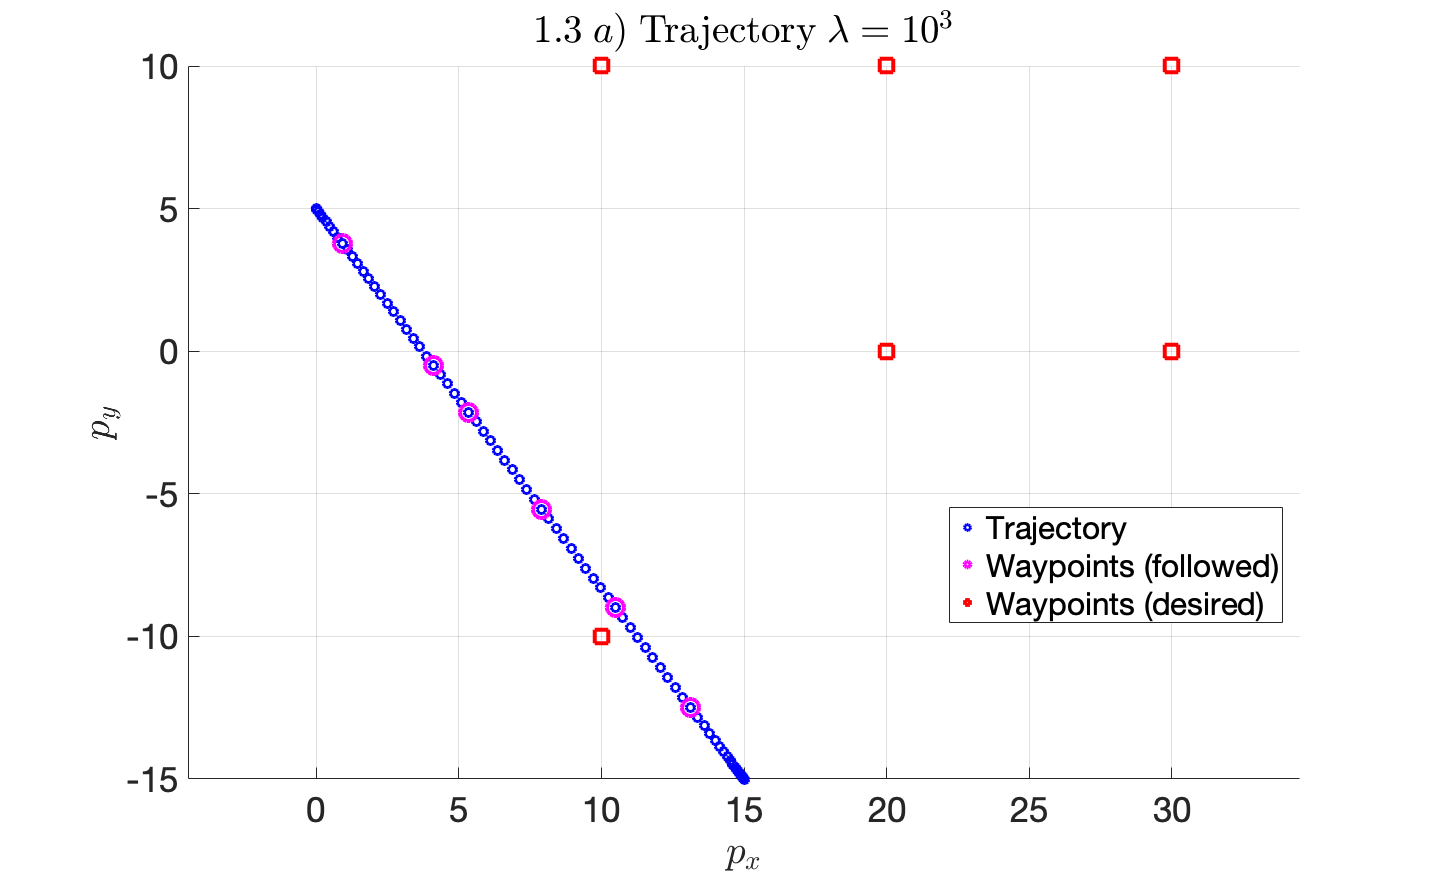
\includegraphics[width=\maxwidth{144.5057701956849em}]{figure_26}
\end{center}

\begin{center}
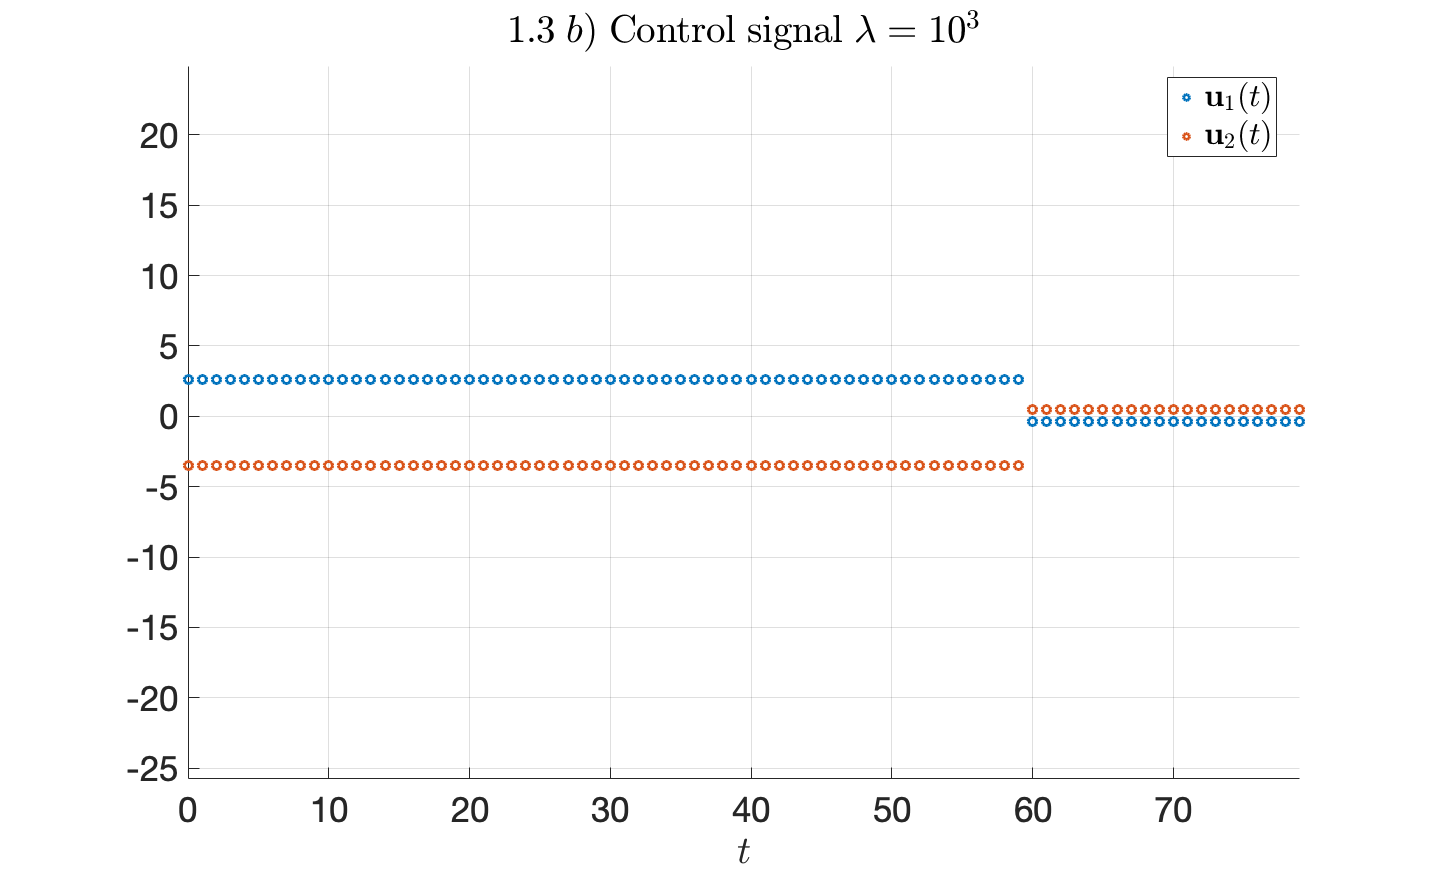
\includegraphics[width=\maxwidth{144.5057701956849em}]{figure_27}
\end{center}
\begin{matlaboutput}
1.3 c) For lambda = 1e3 there were 1 optimal control signal changes.
1.3 c) For lambda = 1e3 there were 1 optimal control signal L1 changes.
1.3 d) For lambda = 1e3 the mean deviation from the waypoints is 16.226625.
\end{matlaboutput}
\begin{matlabcode}
save('./transferring_a_robot_data/1_3_data_c_d.mat','controlSignalChanges','controlSignalChangesL1','meanDeviation');

\end{matlabcode}


\matlabheading{1.4 The $l_1$ regularizer}

\begin{matlabcode}
controlSignalChanges = [];
controlSignalChangesL1 = [];
meanDeviation = [];

for lambda_log = -3:3
    % ---------- Setup optimization problem ----------
    cvx_begin quiet
        % optimization variables
        variables x(n,T+1) u(m,T)
        % cost function
        minimize(sum(sum_square(E*x(:,tau+1)-w))+...
            (10^lambda_log)*sum(norms(u*(diag(-[ones(T-1,1);0])+diag(ones(T-1,1),-1)),1)));
        % subject to
        x(:,1) == [p_initial;zeros(2,1)];
        x(:,end) == [p_final;zeros(2,1)];
        for t = 1:T
            x(:,t+1) == A*x(:,t)+B*u(:,t);
            norm(u(:,t)) <= U_max;
        end
    cvx_end
    
    % ---------- Plot result ----------
    % trajectory
    figure('units','normalized','outerposition',[0 0 1 1]);
    hold on;
    set(gca,'FontSize',35);
    ax = gca;
    ax.XGrid = 'on';
    ax.YGrid = 'on';
    axis equal;
    title(strcat('$1.4\;a)\; \mathrm{Trajectory}\;\lambda =',sprintf('10^{%d}$',lambda_log)),'Interpreter','latex');
    scatter(x(1,:),x(2,:),70,'o','blue','LineWidth',3);
    scatter(x(1,tau+1),x(2,tau+1),300,'o','magenta','LineWidth',4);
    scatter(w(1,:),w(2,:),300,'s','red','LineWidth',4);
    legend('Trajectory','Waypoints (followed)', 'Waypoints (desired)','Location','best');
    ylabel('$p_y$','Interpreter','latex');
    xlabel('$p_x$','Interpreter','latex');
    saveas(gcf,sprintf('./transferring_a_robot_data/1_4_trajectory_1e%d.fig',lambda_log));
    saveas(gcf,sprintf('./transferring_a_robot_data/1_4_trajectory_1e%d.png',lambda_log));
    hold off; 
    
    % control signal
    figure('units','normalized','outerposition',[0 0 1 1]);
    hold on;
    set(gca,'FontSize',35);
    ax = gca;
    ax.XGrid = 'on';
    ax.YGrid = 'on';
    axis equal;
    title(strcat('$1.4\;b)\; \mathrm{Control}\;\mathrm{signal}\;\lambda =',sprintf('10^{%d}$',lambda_log)),'Interpreter','latex');
    scatter(0:T-1,u(1,:),70,'o','LineWidth',3);
    scatter(0:T-1,u(2,:),70,'o','LineWidth',3);
    legend({'$\mathbf{u}_1(t)$','$\mathbf{u}_2(t)$'},'Location','best','interpreter','latex');
    ylabel('$ $','Interpreter','latex');
    xlabel('$t$','Interpreter','latex');
    saveas(gcf,sprintf('./transferring_a_robot_data/1_4_controlSignal_1e%d.fig',lambda_log));
    saveas(gcf,sprintf('./transferring_a_robot_data/1_4_controlSignal_1e%d.png',lambda_log));
    hold off;
    
    controlSignalChangesCur = 0;
    for t = 1:T-1
        if norm(u(:,t+1)-u(:,t))>1e-4
            controlSignalChangesCur = controlSignalChangesCur+1;
        end
    end
    controlSignalChanges = [controlSignalChanges [10^lambda_log;controlSignalChangesCur]]; 
    fprintf("1.4 c) For lambda = 1e%d there were %d optimal control signal changes.\n",lambda_log,controlSignalChangesCur);
    
    controlSignalChangesCurL1 = 0;
    for t = 1:T-1
        if norms(u(:,t+1)-u(:,t),1)>1e-4
            controlSignalChangesCurL1 = controlSignalChangesCurL1+1;
        end
    end
    controlSignalChangesL1 = [controlSignalChangesL1 [10^lambda_log;controlSignalChangesCurL1]]; 
    fprintf("1.4 c) For lambda = 1e%d there were %d optimal control signal L1 changes.\n",lambda_log,controlSignalChangesCurL1);    
    
    meanDeviationCur = (1/length(w))*sum(sqrt(sum_square(E*x(:,tau+1)-w)));
    meanDeviation = [meanDeviation [10^lambda_log; meanDeviationCur]];
    fprintf("1.4 d) For lambda = 1e%d the mean deviation from the waypoints is %f.\n",lambda_log,meanDeviationCur);
    
end
\end{matlabcode}
\begin{center}
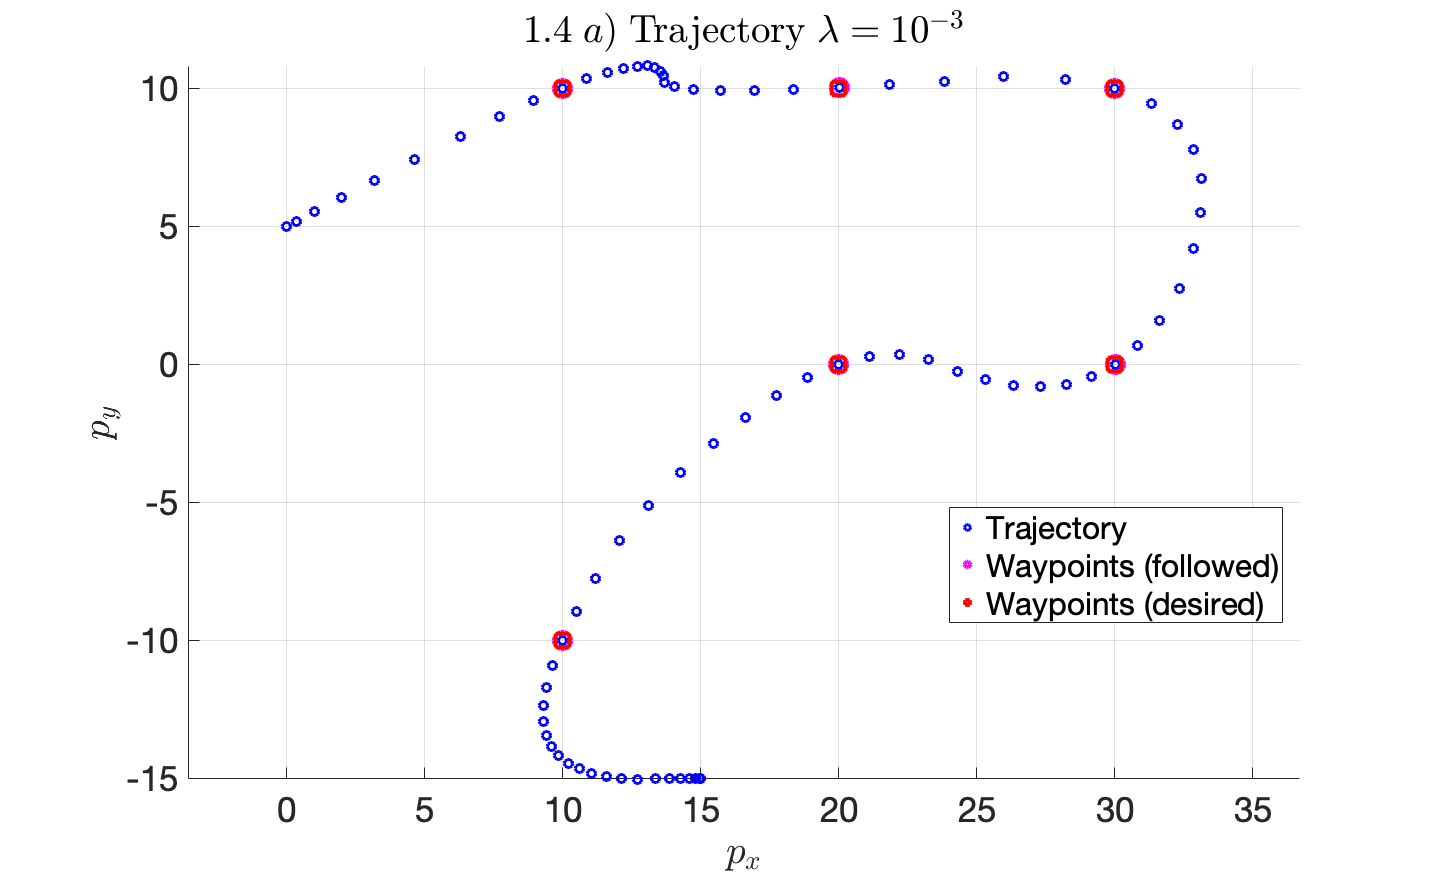
\includegraphics[width=\maxwidth{144.5057701956849em}]{figure_28}
\end{center}

\begin{center}
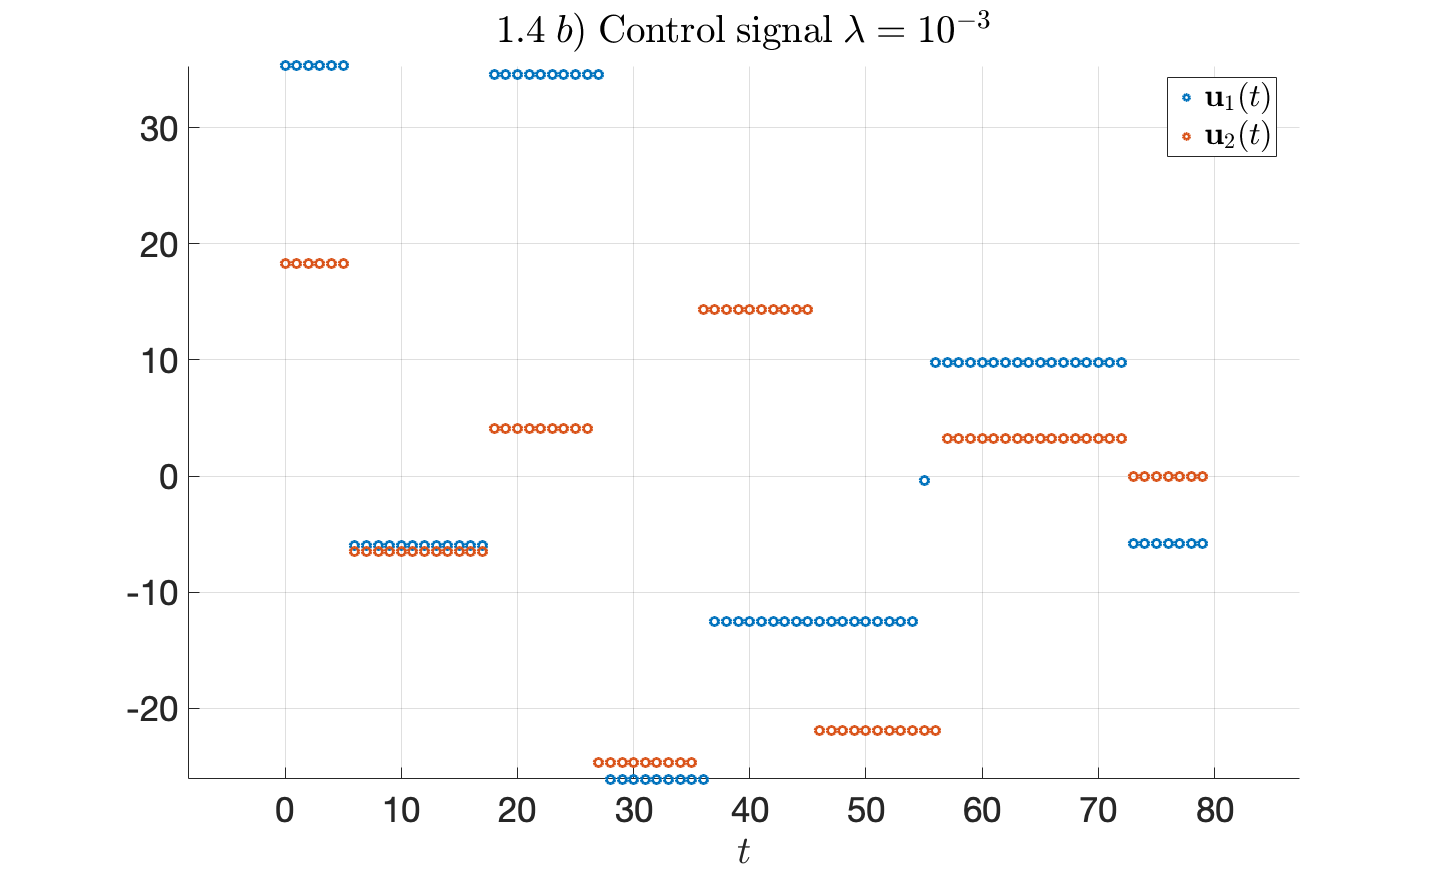
\includegraphics[width=\maxwidth{144.5057701956849em}]{figure_29}
\end{center}
\begin{matlaboutput}
1.4 c) For lambda = 1e-3 there were 11 optimal control signal changes.
1.4 c) For lambda = 1e-3 there were 11 optimal control signal L1 changes.
1.4 d) For lambda = 1e-3 the mean deviation from the waypoints is 0.010735.
\end{matlaboutput}
\begin{center}
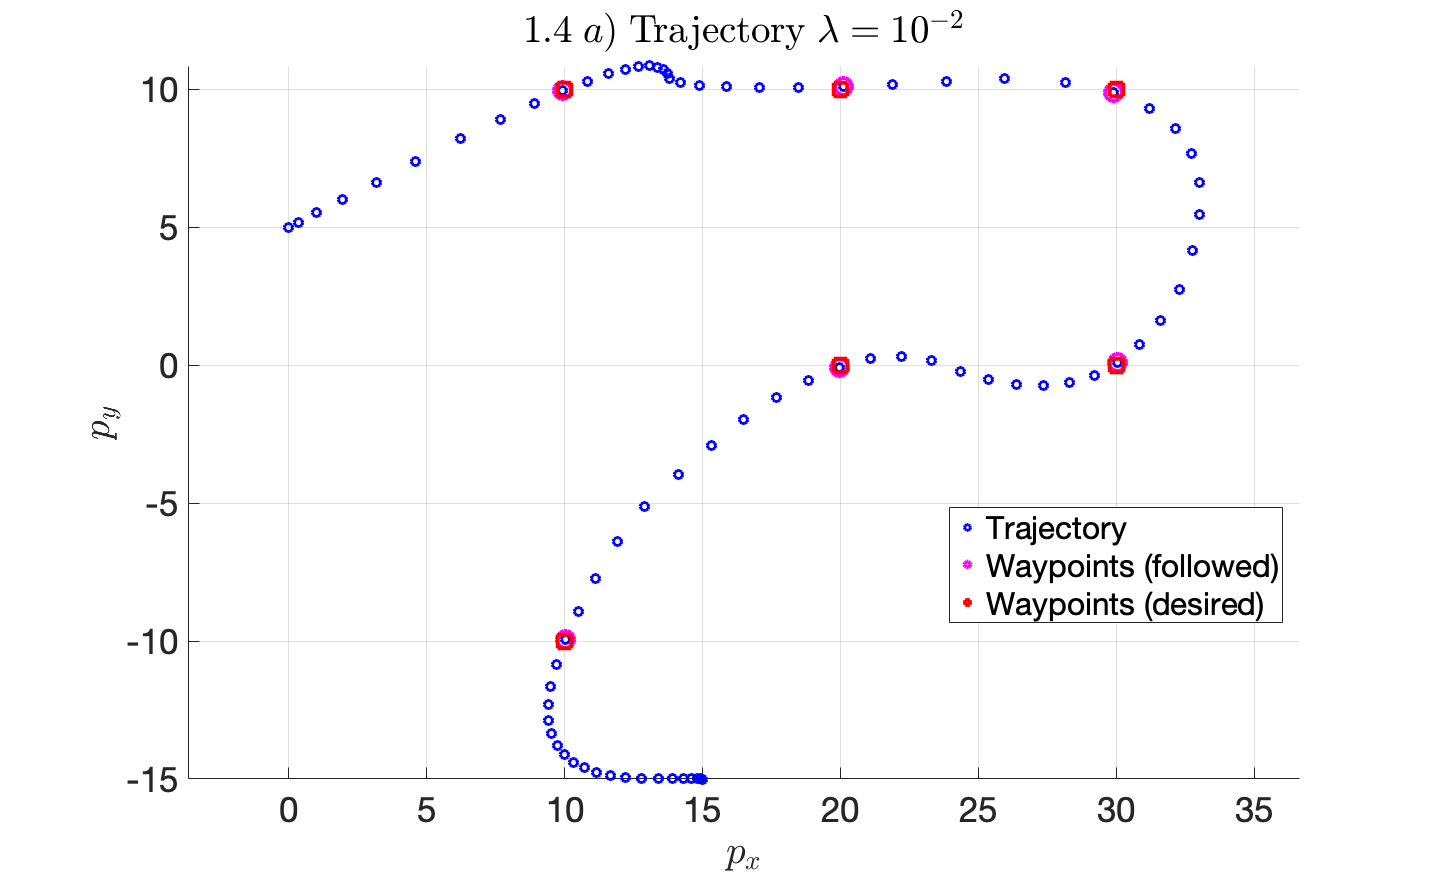
\includegraphics[width=\maxwidth{144.5057701956849em}]{figure_30}
\end{center}

\begin{center}
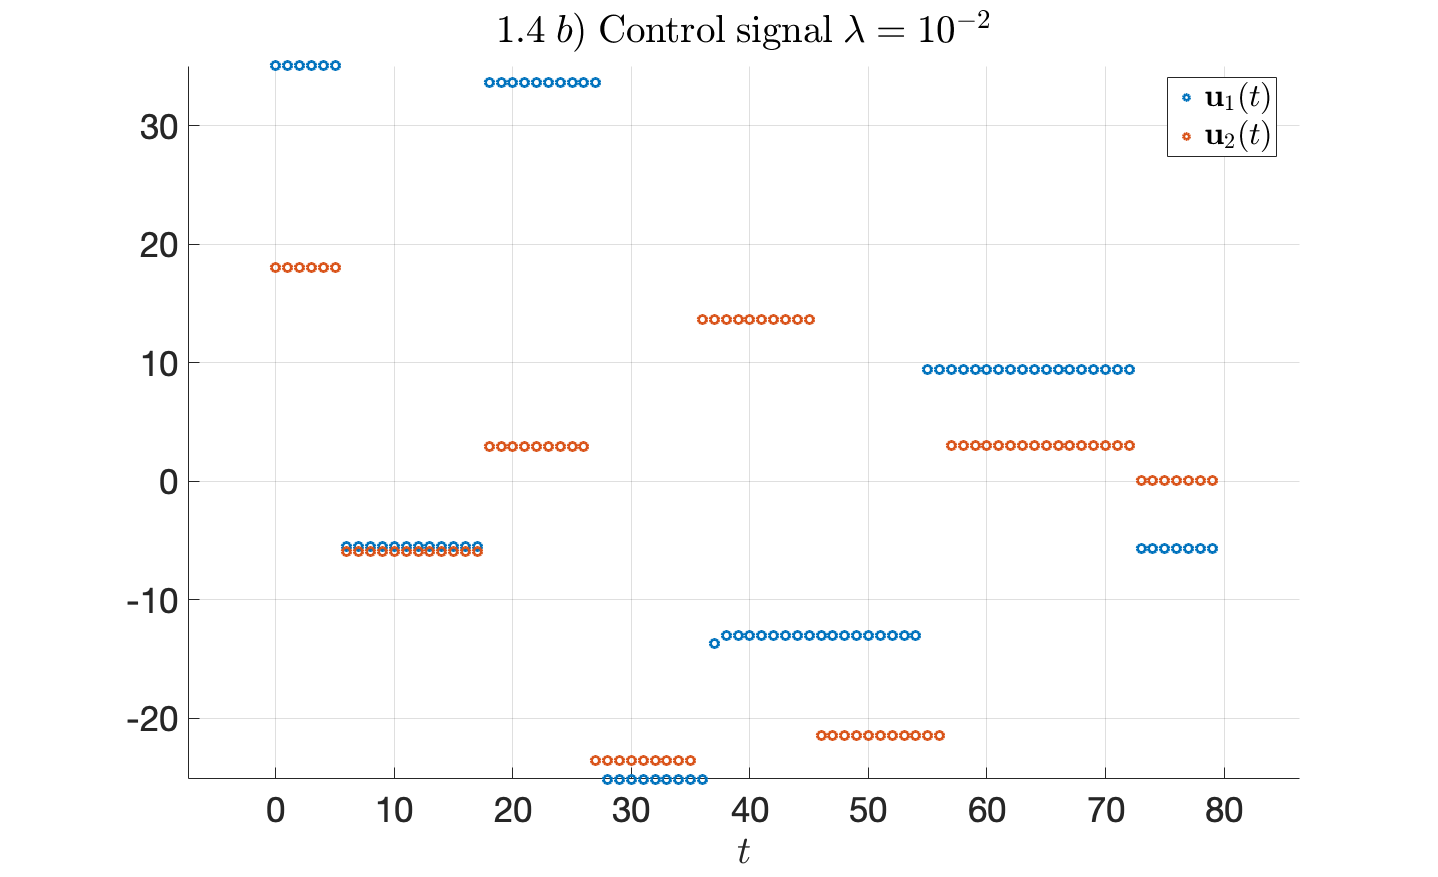
\includegraphics[width=\maxwidth{144.5057701956849em}]{figure_31}
\end{center}
\begin{matlaboutput}
1.4 c) For lambda = 1e-2 there were 11 optimal control signal changes.
1.4 c) For lambda = 1e-2 there were 11 optimal control signal L1 changes.
1.4 d) For lambda = 1e-2 the mean deviation from the waypoints is 0.105450.
\end{matlaboutput}
\begin{center}
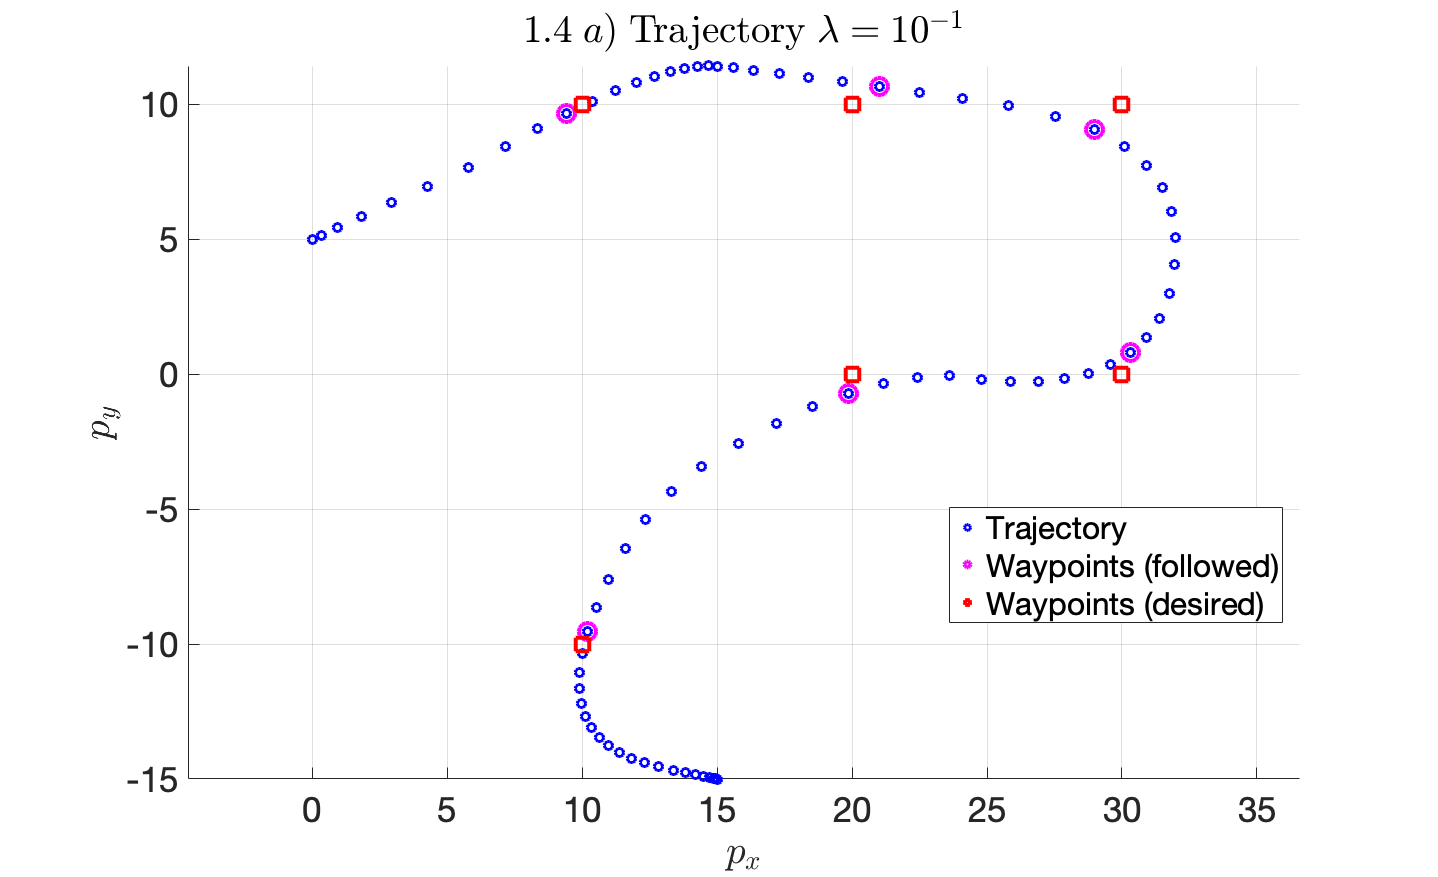
\includegraphics[width=\maxwidth{144.5057701956849em}]{figure_32}
\end{center}

\begin{center}
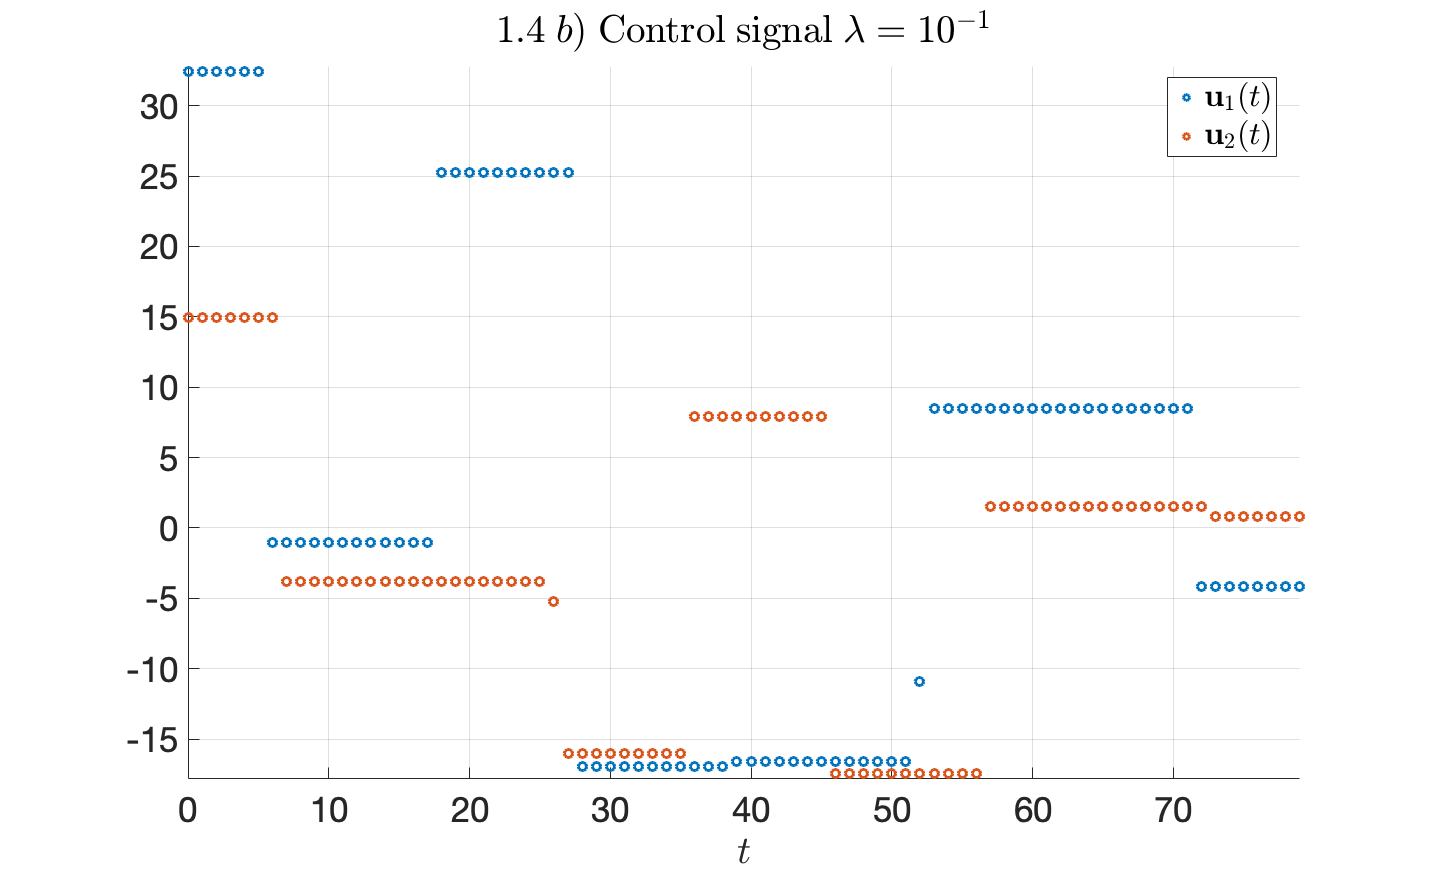
\includegraphics[width=\maxwidth{144.5057701956849em}]{figure_33}
\end{center}
\begin{matlaboutput}
1.4 c) For lambda = 1e-1 there were 14 optimal control signal changes.
1.4 c) For lambda = 1e-1 there were 14 optimal control signal L1 changes.
1.4 d) For lambda = 1e-1 the mean deviation from the waypoints is 0.886316.
\end{matlaboutput}
\begin{center}
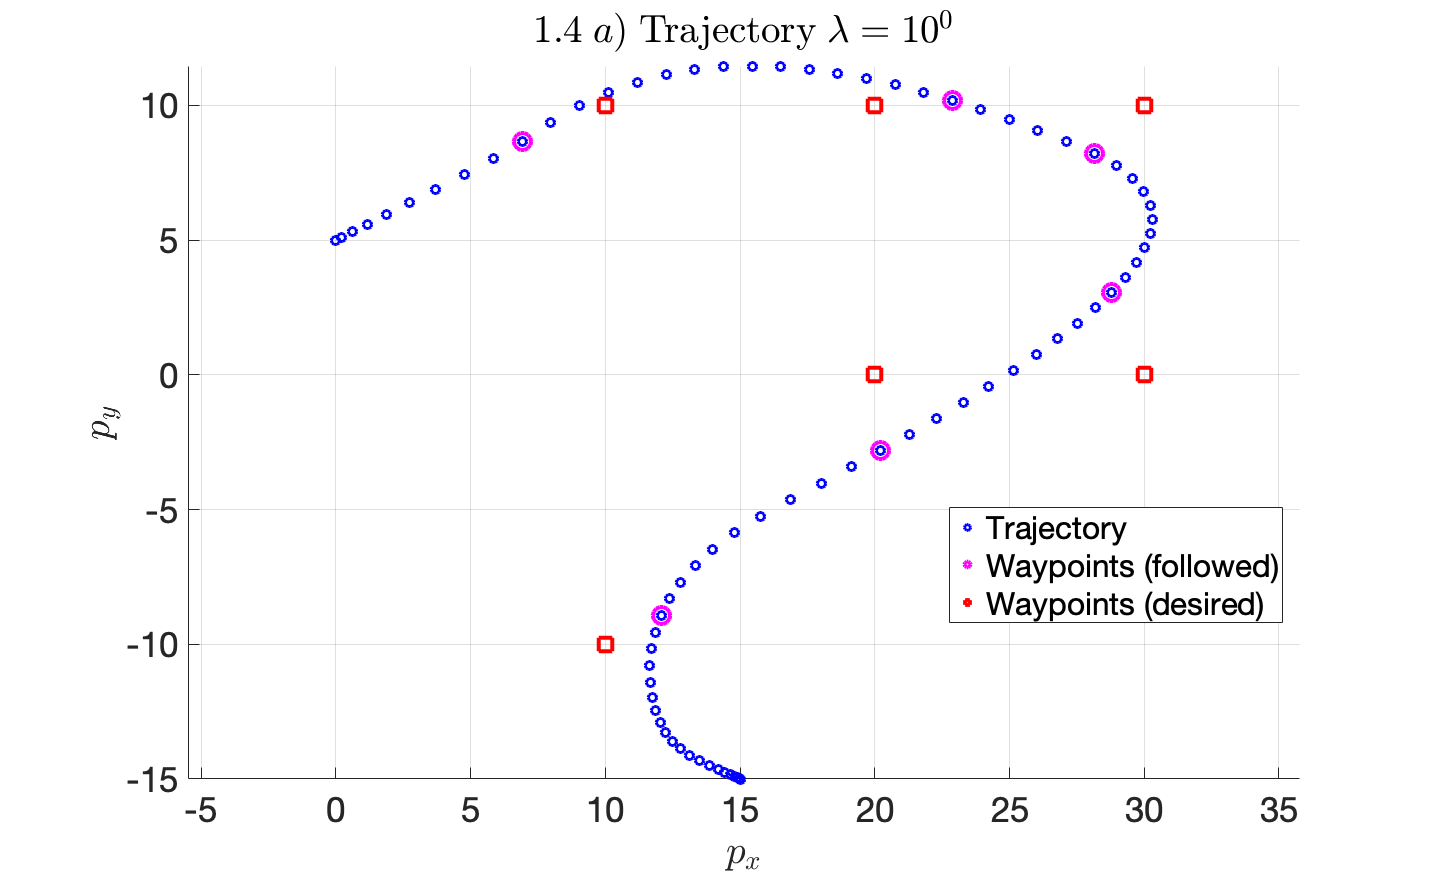
\includegraphics[width=\maxwidth{144.5057701956849em}]{figure_34}
\end{center}

\begin{center}
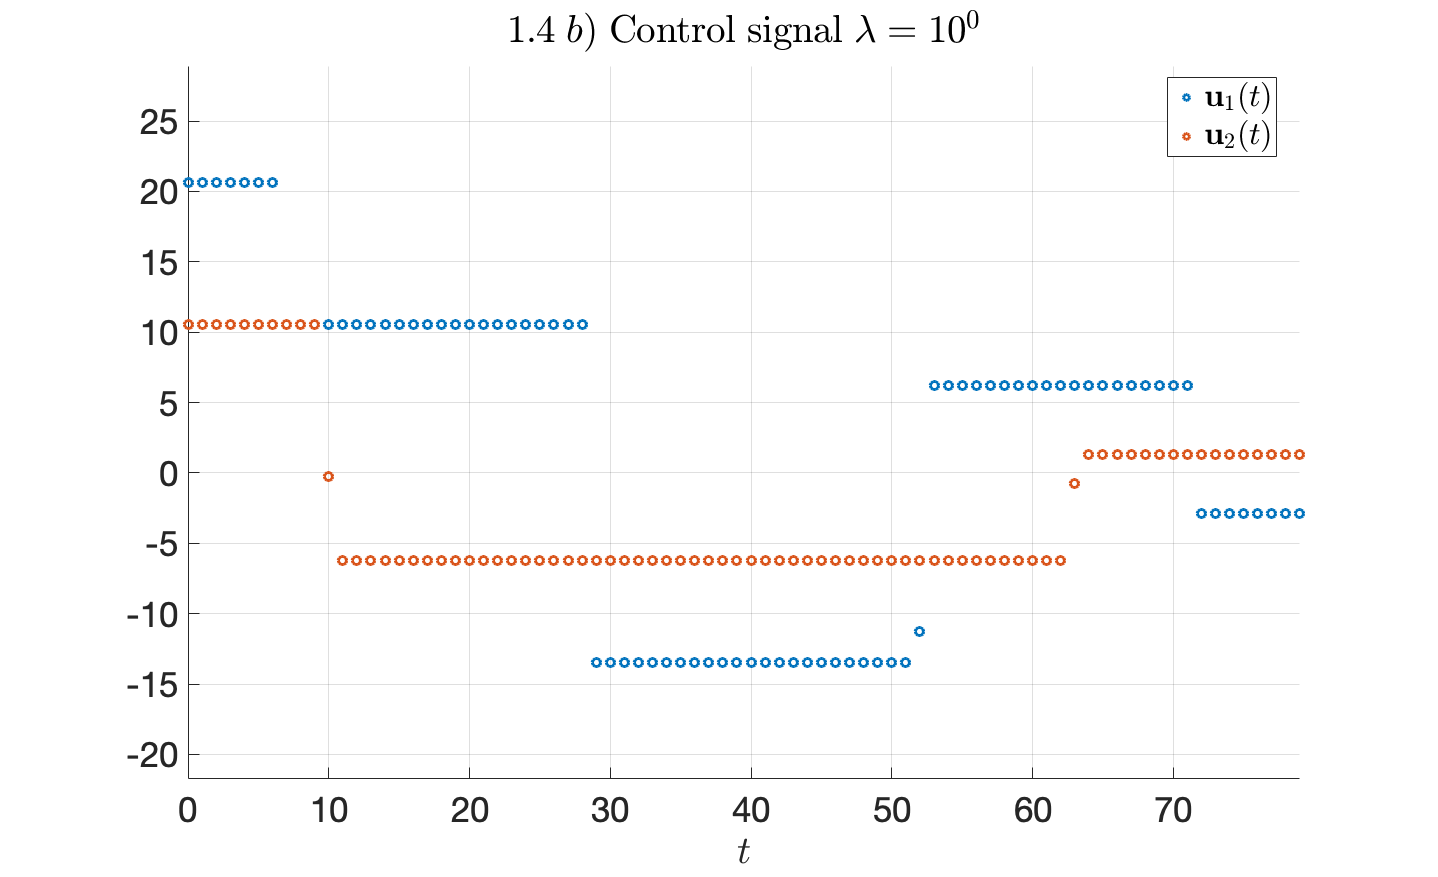
\includegraphics[width=\maxwidth{144.5057701956849em}]{figure_35}
\end{center}
\begin{matlaboutput}
1.4 c) For lambda = 1e0 there were 9 optimal control signal changes.
1.4 c) For lambda = 1e0 there were 9 optimal control signal L1 changes.
1.4 d) For lambda = 1e0 the mean deviation from the waypoints is 2.873231.
\end{matlaboutput}
\begin{center}
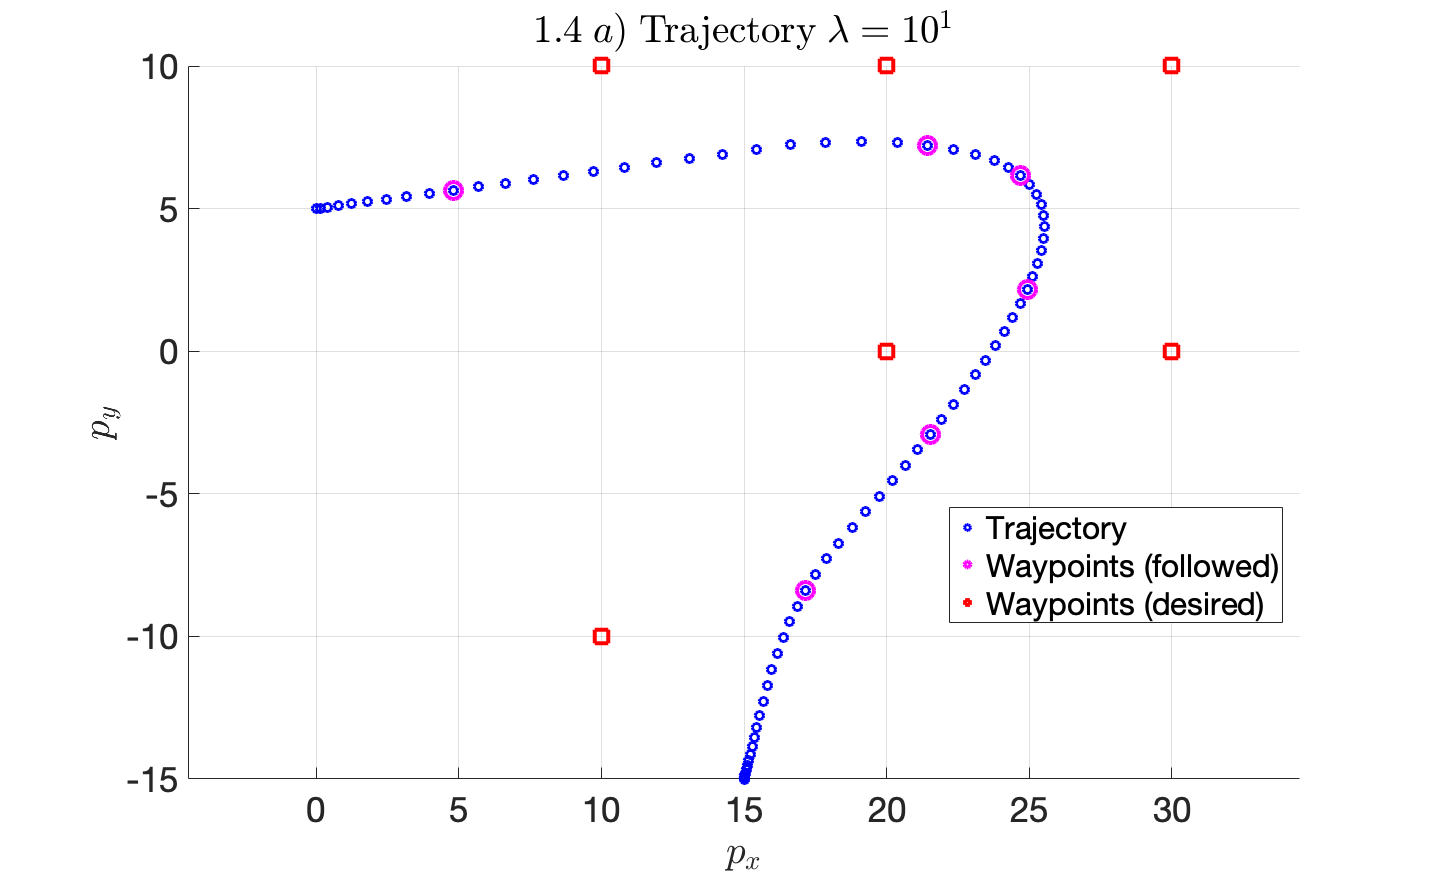
\includegraphics[width=\maxwidth{144.5057701956849em}]{figure_36}
\end{center}

\begin{center}
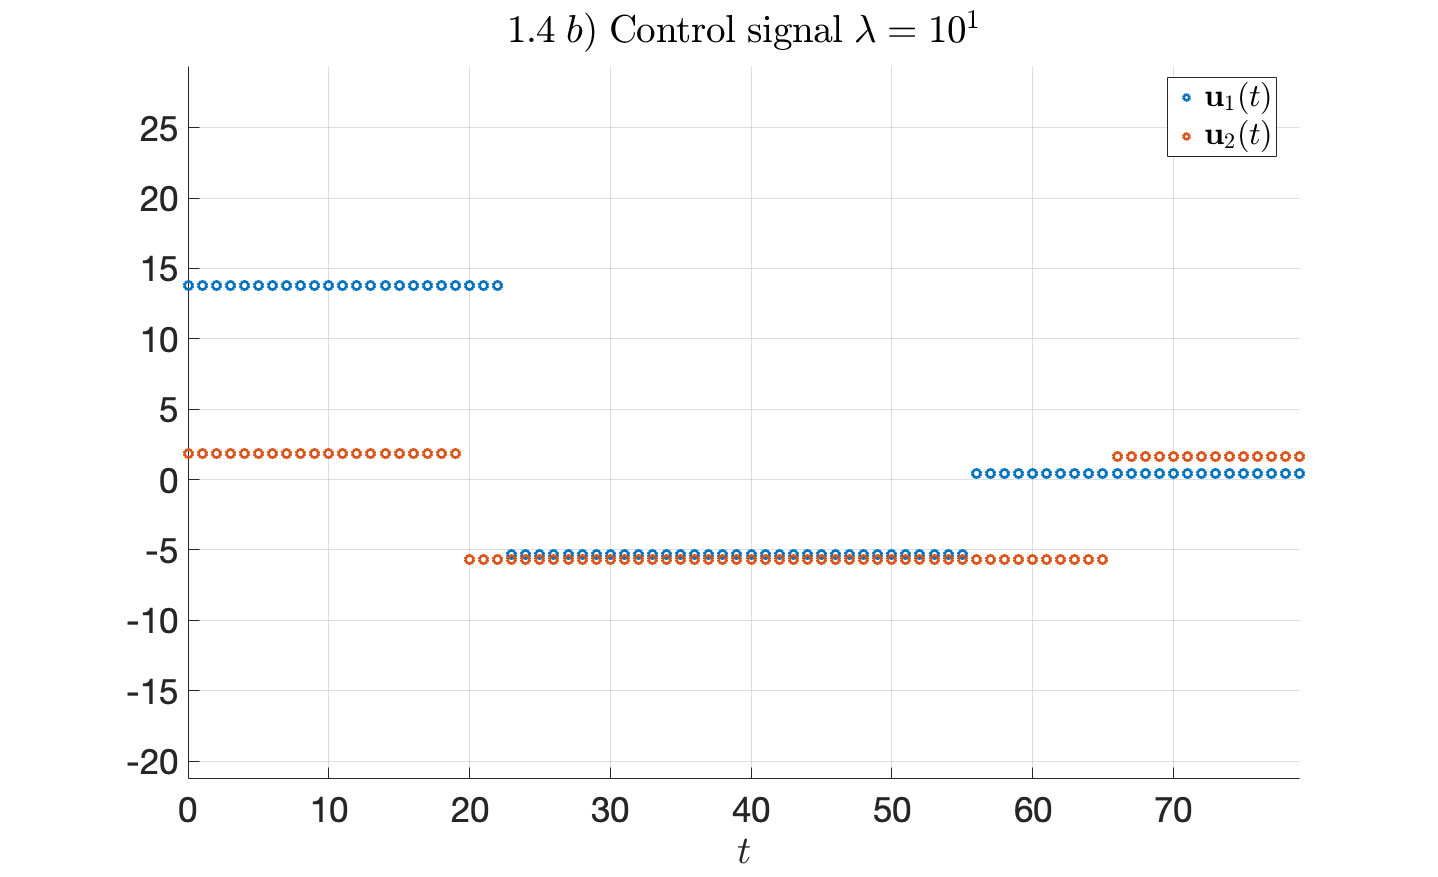
\includegraphics[width=\maxwidth{144.5057701956849em}]{figure_37}
\end{center}
\begin{matlaboutput}
1.4 c) For lambda = 1e1 there were 4 optimal control signal changes.
1.4 c) For lambda = 1e1 there were 4 optimal control signal L1 changes.
1.4 d) For lambda = 1e1 the mean deviation from the waypoints is 5.436149.
\end{matlaboutput}
\begin{center}
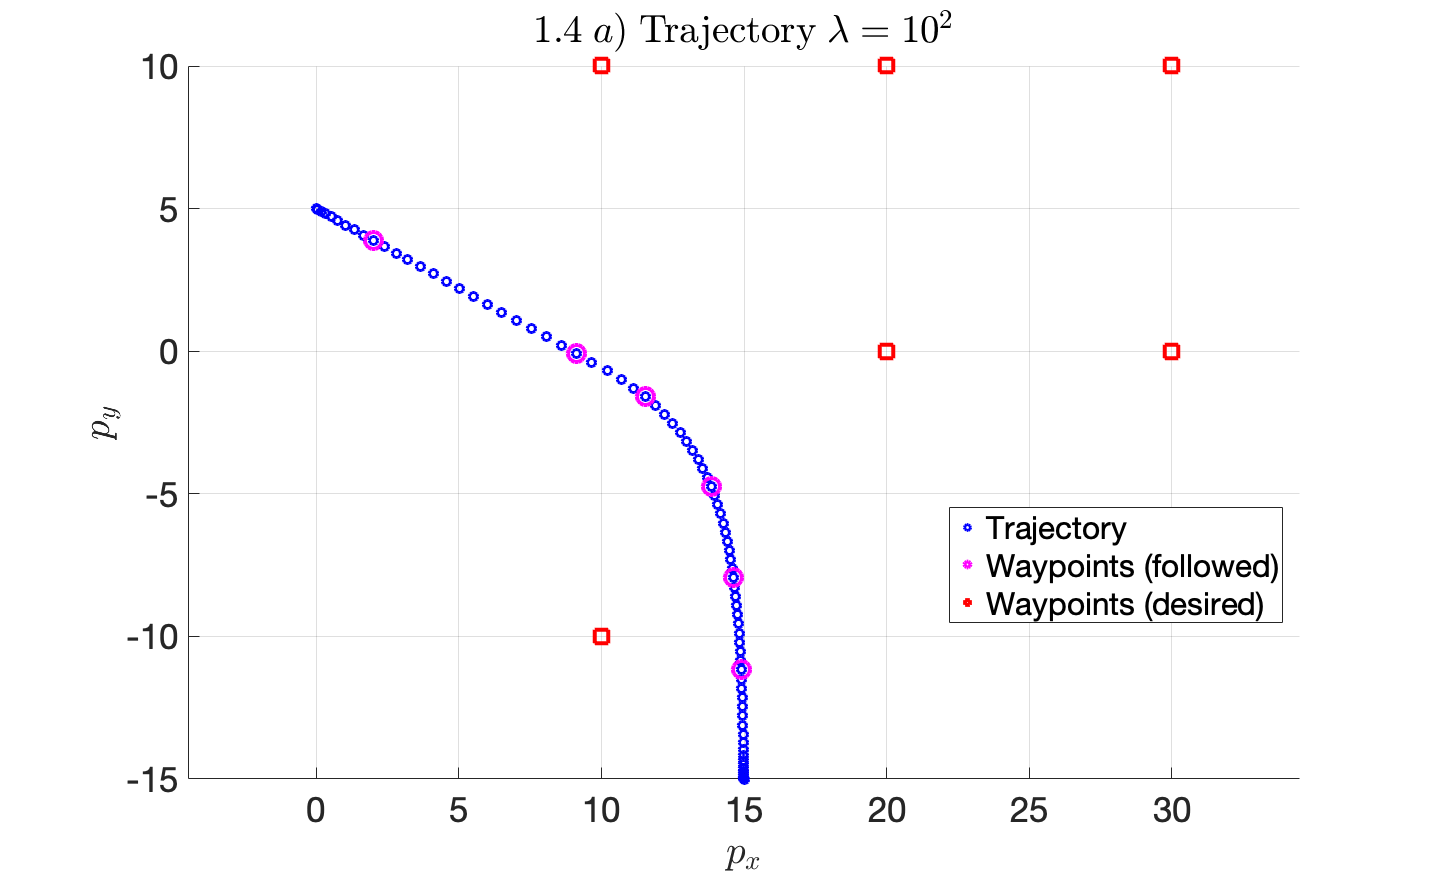
\includegraphics[width=\maxwidth{144.5057701956849em}]{figure_38}
\end{center}

\begin{center}
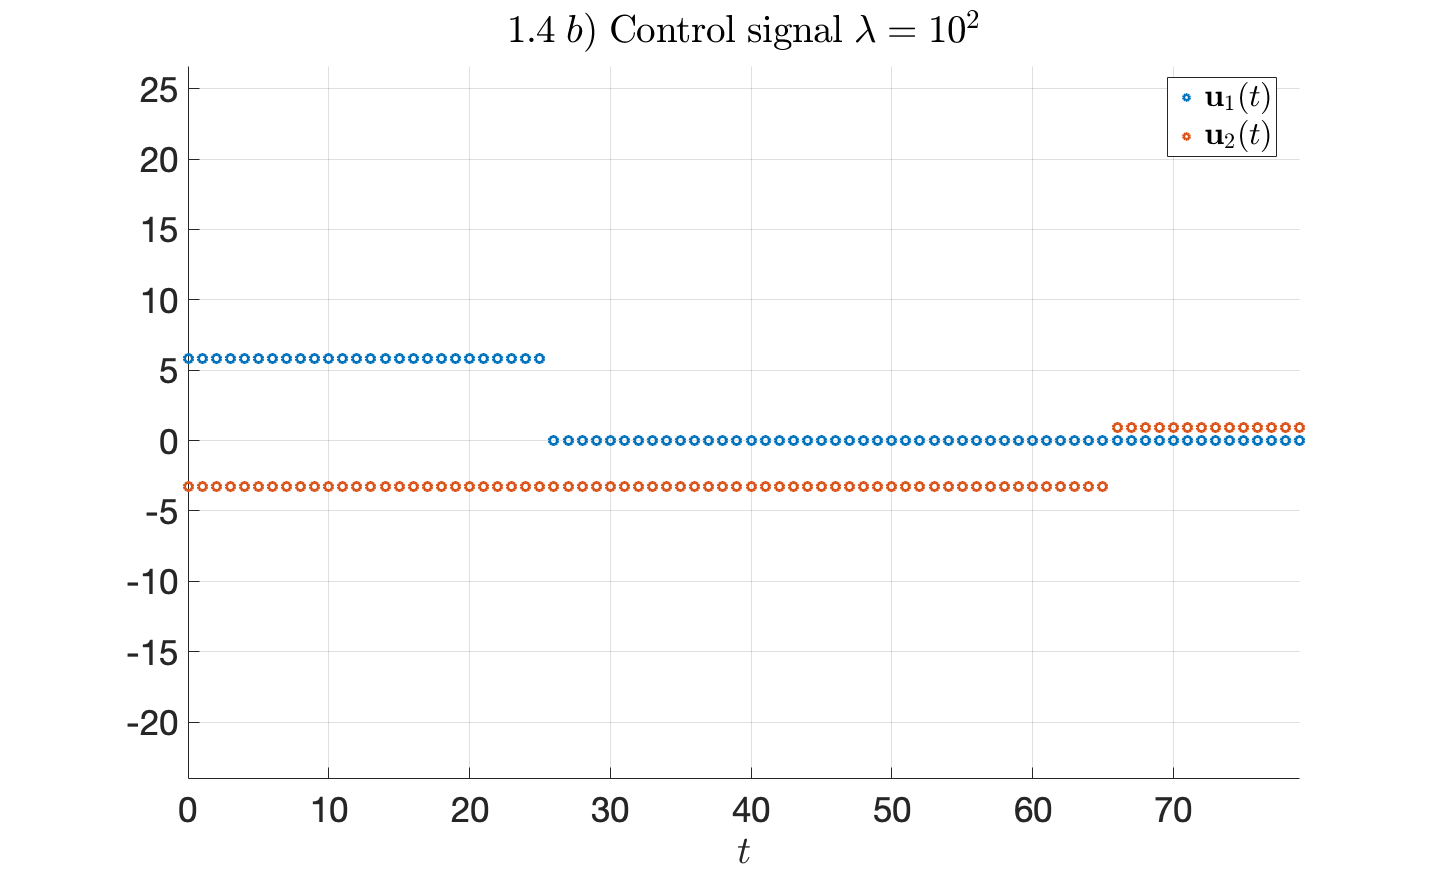
\includegraphics[width=\maxwidth{144.5057701956849em}]{figure_39}
\end{center}
\begin{matlaboutput}
1.4 c) For lambda = 1e2 there were 2 optimal control signal changes.
1.4 c) For lambda = 1e2 there were 2 optimal control signal L1 changes.
1.4 d) For lambda = 1e2 the mean deviation from the waypoints is 13.027273.
\end{matlaboutput}
\begin{center}
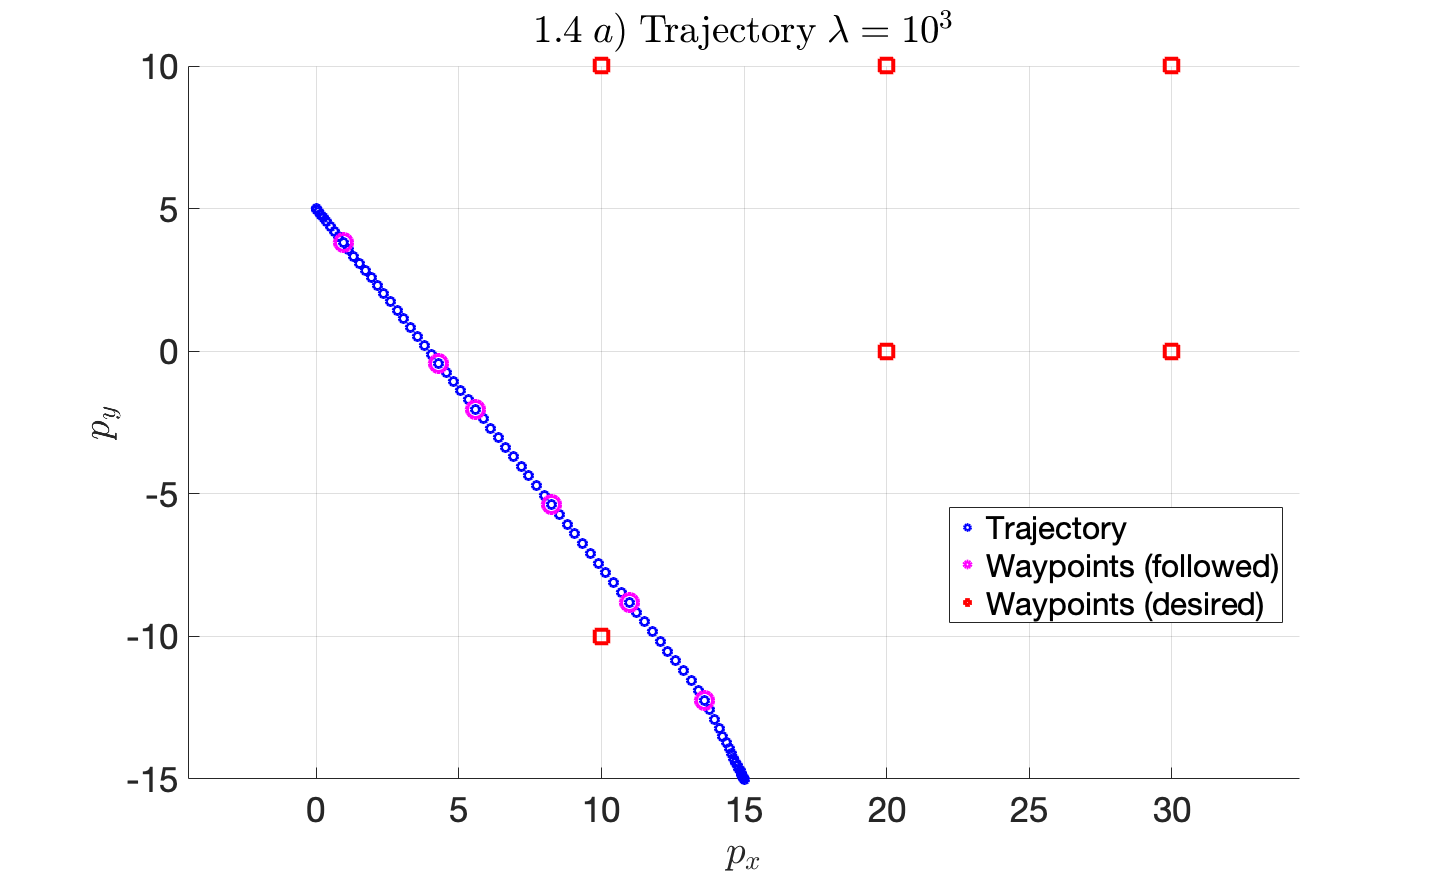
\includegraphics[width=\maxwidth{144.5057701956849em}]{figure_40}
\end{center}

\begin{center}
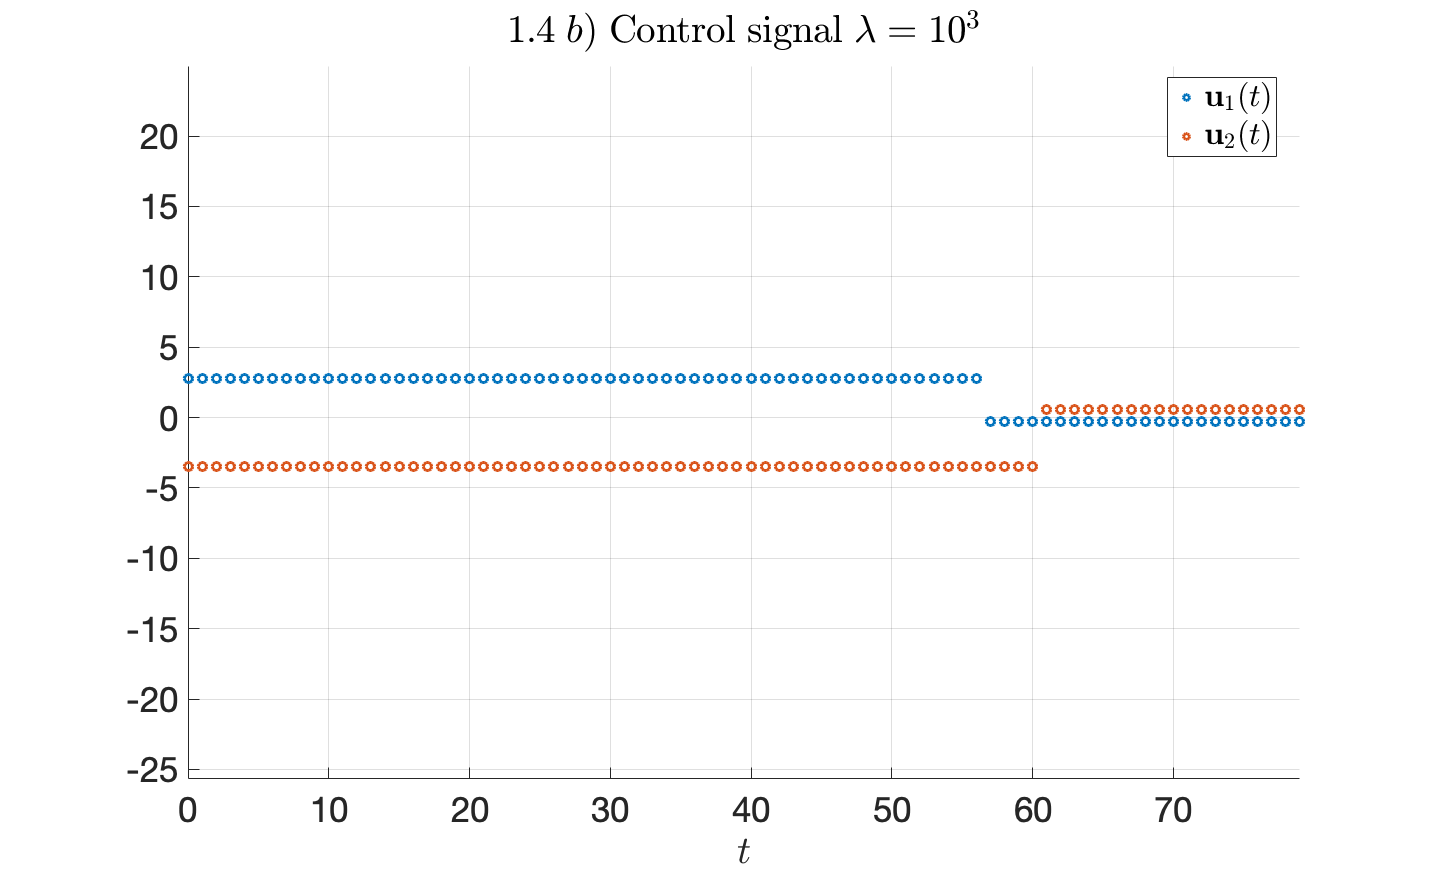
\includegraphics[width=\maxwidth{144.5057701956849em}]{figure_41}
\end{center}
\begin{matlaboutput}
1.4 c) For lambda = 1e3 there were 2 optimal control signal changes.
1.4 c) For lambda = 1e3 there were 2 optimal control signal L1 changes.
1.4 d) For lambda = 1e3 the mean deviation from the waypoints is 16.046286.
\end{matlaboutput}
\begin{matlabcode}
save('./transferring_a_robot_data/1_4_data_c_d.mat','controlSignalChanges','meanDeviation','controlSignalChangesL1');
\end{matlabcode}


\matlabheading{Comments}

\begin{par}
\begin{flushleft}
"Task 4. Comment on what you have observed from Tasks 1 to 3 (for example, compare the impact of the three regularizers on the optimal control signal that they each induce)."
\end{flushleft}
\end{par}

\vspace{1em}

\begin{par}
\begin{flushleft}
Mean deviation from waypoints
\end{flushleft}
\end{par}

\begin{par}
$$\lambda$$       $$10^{-3}$$        $$10^{-2}$$       $$10^{-1}$$       $$10^{0}$$         $$10^{1}$$        $$10^{2}$$          $$10^{3}$$
\end{par}

\begin{par}
\begin{flushleft}
$l_2^2$       0.1257    0.8242    2.1958    3.6826    5.6317   10.9041   15.3304
\end{flushleft}
\end{par}

\begin{par}
\begin{flushleft}
$l_2$       0.0075    0.0747    0.7021    2.8876    5.3689   12.5914   16.2266
\end{flushleft}
\end{par}

\begin{par}
\begin{flushleft}
$l_1$       0.0107    0.1055    0.8863    2.8732    5.4361   13.0273   16.0463
\end{flushleft}
\end{par}

\vspace{1em}

\begin{par}
\begin{flushleft}
Number of changes (L2) in the optimal control signal
\end{flushleft}
\end{par}

\begin{par}
$$\lambda$$       $$10^{-3}$$        $$10^{-2}$$       $$10^{-1}$$       $$10^{0}$$         $$10^{1}$$        $$10^{2}$$          $$10^{3}$$
\end{par}

\begin{par}
\begin{flushleft}
$l_2^2$       79            79           79          79           79          79            79
\end{flushleft}
\end{par}

\begin{par}
\begin{flushleft}
$l_2$      10             8             10          5             4            3              1
\end{flushleft}
\end{par}

\begin{par}
\begin{flushleft}
$l_1$      13             12           14          9             6            3              3
\end{flushleft}
\end{par}

\vspace{1em}

\begin{par}
\begin{flushleft}
First, it is possible to notice that using the $l_2^2$ regularizer, whatever the value of $\lambda$ is there is always the maximum number of changes of the optimal control signal. Using this regularizer, the optimal control obtained is a smooth continuous signal. In fact, the weighing factor is the square of the difference. Once the difference is low (\textless{}\textless{}1) the square reduces this difference even more. This way, this regularizer penalizes very significantly big differences, but is benevolent when the diffferences are small. This behaviour is not ideal for problems where there may be outliers, which is not the case. This originates a smooth signal.
\end{flushleft}
\end{par}

\begin{par}
\begin{flushleft}
Second, both the $l_2$ and $l_1$ regularizers do not penalize big differences significantly and are not as benevolent with small differences, as it is the case with the $l_2^2$ regularizer. In fact, this results, for both aproaches in a roughly piecewise constant signal for every  value of $\lambda$. Given that the $||x||_1 \geq ||x||_2$, then, for the same value of $\lambda$ it is expected that the $l_1$ regularizer penallizes changes in the optimal control signal more than the $l_2$ regularizer. As expected, given that more importance is given to the regularizer, the performance as far as waypoint tracking is concerned decreases slightly for the $l_1$ regularizer when compared with the $l_2$ regularizer. Furthermore, it is also notiable that the $l_1$ norm, also because of the aforementioned increse of regularizer importance and the fact that it is the sum of the absloute values of the components of a vector, is more prone to originate sparse control signals.
\end{flushleft}
\end{par}

\end{document}
